\documentclass{article}
\usepackage[most]{tcolorbox}
\usepackage{xcolor, array}
\usepackage[table]{xcolor}
\usepackage{graphicx, float}
\usepackage[T1]{fontenc}
\usepackage[utf8]{inputenc}
\usepackage[sfdefault]{atkinson}
\graphicspath{{images/}}
\usepackage{amsthm, amssymb, amsmath}
\usepackage[a4paper]{geometry}
\usepackage[dvipsnames]{xcolor}
\usepackage[skip=8pt, indent= 0pt]{parskip}
\usepackage{pgfplots}
\usepackage[hidelinks]{hyperref}
\usepackage{cancel}
\pgfplotsset{compat=1.18, width=10cm}
\geometry{
a4paper,
total={170mm,257mm},
left=20mm,
top=20mm,
}
\title{Analisi Matematica}
\author{Marco Pittarello}
\date{}

\newtcbtheorem{theo}{Teorema}{%
    colframe=BrickRed!100!white,
    colback=red!5!white
}{th}

\newtcbtheorem{ex}{Esempio}{%
    colframe=OliveGreen!100!white,
    colback=OliveGreen!5!white
}{ex}

\newtcbtheorem{defi}{Definizione}{%
    colframe=blue!100!white,
    colback=blue!10!white
}{def}
\renewcommand{\arraystretch}{2}
\setlength{\tabcolsep}{20pt}
\begin{document}
\maketitle
\tableofcontents
\newpage
\section{Principio di Induzione}

\begin{defi}{}{}
Il principio di induzione è un metodo per dimostrare predicati matematici.
\end{defi}
come \\
\begin{itemize}
    \item []$\forall n \in \mathbb{N} \qquad \underbrace{1 + 2 + 3 + \dots + n \ = \ \frac{n\ (n+1)}{2}}_{\text{P}(n)}$\\
    \item []$\forall n \in \mathbb{N} \qquad \underbrace{\forall x \in \mathbb{R} \quad x >  1 \quad (1+x)^n \ge nx+1}_{\text{P}(n)}$
\end{itemize}
\begin{theo}{1° forma}{}
Sia P$(n)$ un predicato con parametro $n \in \mathbb{N}$ e tale che:
\begin{enumerate}
    \item P$(0)$ è vero (\colorbox{yellow}{caso base})
    \item $\forall n \in \mathbb{N}\quad \text{P}(n) \xrightarrow{}\text{P}(n+1)$ (\colorbox{yellow}{passo induttivo})
\end{enumerate}
Allora $P(n)$ è vera $\forall n \in \mathbb{N}$
\end{theo}\ 

\begin{ex}{}{}
Dimostrare che $\forall n \in \mathbb{N} \quad \underbrace{2^n \ge n+1}_{\text{P}(n)}$.
\end{ex}
\underline{CASO BASE} : \quad P$(0) \quad 2^0 \ge 1 \quad \text{vero}$

\underline{PASSO INDUTTIVO} : \quad  $\forall n \in \mathbb{N} \quad \text{P}(n) \xrightarrow{} \text{P}(n+1)$\\

\begin{itemize}
    \item[] Suppongo che $2^n \ge n+1$ e dimostro che $2^{n+1} \ge n +2$
    \item[] $2^n \ge n+1\ \xrightarrow{}\ 2\cdot 2^n \ge 2 \cdot (n+1) $
    \item[] $2^{n+1}\ \ge\ 2n+2\ge n+2$
    \item[] Dunque abbiamo dimostrato che P$(n)\xrightarrow{}\text{P}(n+1)$
    \item[] Dunque per il principio di induzione è vero che $\forall n \in \mathbb{N}$ vale P$(n)$\\
\end{itemize}

\begin{ex}{}{}
    Dimostrare che $\forall n \in \mathbb{N}$ : \[\sum^n_{k=0}k = \frac{n(n+1)}{2}\]
\end{ex}
\underline{CASO BASE} : P$(0):\ $"$0$ = $0$" è vera

\underline{PASSO INDUTTIVO} :\quad Assumo che P$(n)$ è vera e dimostro che è vera anche P$(n+1)$

    \[\text{ovvero}\qquad \sum^{n+1}_{k=0}k=\frac{(n+1)(n+2)}{2}\]

    \[\sum^{n+1}_{k=0}k=\ \sum^{n}_{k=0}k+(n+1)\ =\ \frac{n(n+1)}{2}+(n+1)=\ \frac{n(n+1)+2(n+1)}{2}=\ \frac{(n+2)(n+1)}{2}\]
Ho dimostrato CASO BASE e PASSO INDUTTIVO, dunque per il principio di induzione segue che: 
\[\forall n\in\mathbb{N}\quad \text{P}(n)\]
\begin{theo}{2° forma}{}
    Sia P$(n)$, $n \in\mathbb{N}$\quad un predicato tale che:
    \begin{enumerate}
        \item P$(0)$ è vera (\colorbox{yellow}{caso base})
        \item $\forall n\in\mathbb{N}$,\quad $n \ge 1$ (\colorbox{yellow}{passo induttivo})
    \end{enumerate}
    Se $\forall m\in\mathbb{N}\quad 0 \le m \le n\quad \text{P}(n)$ è vera allora lo è anche P$(m)$ (\colorbox{yellow}{ipotesi induttiva})\\Allora $\forall n\in\mathbb{N}\quad \text{P}(n)\quad $ è vera
\end{theo}
\colorbox{yellow}{OSSERVAZIONE} è una forma "più forte" della 1° forma, poichè per dimostrare P$(n)$ si usa la condizione che P$(m)$ vale per tutti gli $m < n$\\\\
\colorbox{yellow}{OSSERVAZIONE} in entrambe le forme del principio di induzione possiamo sostituire $0$ con qualunque $n_0\in\mathbb{N}$. Ovvero, se per un predicato P$(m)$ dimostriamo:
\begin{itemize}
    \item il caso base per $n_o$
    \item il passo induttivo $\forall n\ge n_0$
\end{itemize}
Allora possiamo concludere che $\forall n\ge n_0 \text{P}(n)$ è vera

\begin{ex}{}{}
    Dimostriamo che $\forall n\in\mathbb{N}\quad n\ge2\quad \underbrace{n\text{ si può scrivere come prodotto di numeri primi}}_{\text{P}(n)}$
\end{ex}
\underline{CASO BASE} : P$(2)$ è banalmente vera: 2 è un numero primo


\underline{PASSO INDUTTIVO} : dimostriamo che $\forall n\in\mathbb{N} \quad n\ge3\quad (\forall\quad1\le m<n\quad\text{P}(m)) \xrightarrow{}\text{P}(n)$
\begin{itemize}
    \item[] Ovvero, assumendo che P$(m)$ vale\quad$\forall\quad1\le m<n$, ovvero si può scrivere come prodotto di primi, dimostriamo che anche $n$ si scrive come prodotto di primi ci sono due casi.
    \item[] Se $n$ è primo allore è chiaramente prodotto di primi
    \item[] Se $n$ non è primo allora è divisibile per un numero $m_1$ con $m_1 \ne n$ e $m_1\ne1$, 
    \item[] in particolare $2\le m_1<n$
    \item[] Dunque $\exists m_2\in\mathbb{N}$ tale che
    \item[] $n=m_1m_2$ con $m_1$,$m_2$ diversi da $m$ e da $1$ 
    \item[] Inoltre $2\le m_2<n$
    \item[] perchè $m_1<n$\qquad$m_1>1$
    \item[] Per l'ipotesi induttiva P$(m_1)$ e P$(m_2)$ sono vere.
\end{itemize}
\section{Coefficenti Binomiali}
\begin{defi}{}{}
    Definiamo C$_{n,k}$ = numero totale di modi possibile, e si chiama:
\begin{itemize}
    \item[] \underline{numero di combinazioni di $n$ elementi di classe $k$} 
\end{itemize}
\vspace{5pt}Spesso C$_{n,k}$ viene anche denotato con il simbolo $\binom{n}{k}$, chiamato
\begin{itemize}
    \item[] \underline{coefficiente binomiale $n$ su $k$}
\end{itemize}
\end{defi}
\colorbox{yellow}{Quanto vale $\binom{n}{k}$?}

\[\forall n\in\mathbb{N}\quad \forall k\in\mathbb{N}\quad k\le n\qquad\binom{n}{k} = C_{n,k} =\frac{n!}{k!\ (n-k)!}\]
\subsection{Proprietà del binomio}
    \begin{theo}{}{}
        $\forall n\in\mathbb{N}\quad\forall k\in\mathbb{N}\quad1\le k\le n$ si ha:\\
        \begin{itemize}
            \item [] $\binom{n+1}{k}=\ \binom{n}{k}+\binom{n}{k-1}$
        \end{itemize}
    \end{theo}
\colorbox{yellow}{OSSERVAZIONE:} Abbiamo un altro metodo per calcolare $\binom{n}{k}\forall n\in\mathbb{N}\quad\forall k\le n$\\
Utilizzando il teorema e $\binom{n}{0}=1$ possiamo calcolare ogni valore di $\binom{n}{k}\quad\forall n\in\mathbb{N}\quad\forall k\le n$, evitando di dover calcolare ogni volta i fattoriali.
\begin{ex}{Triangolo di Tartaglia}{}
    Si costruisce elencando per righe i coefficienti binomiali, la riga $n$ è composta da $\binom{n}{0},\binom{n}{1},\dots,\binom{n}{m}$
\end{ex}
\begin{gather}
    \binom{0}{0} = 1\\
    \binom{1}{0} = 1\qquad\binom{1}{1} = 1\\
    \binom{2}{0}=1\qquad\binom{2}{1}=\ \binom{1}{0}+\binom{1}{2}=2\qquad\binom{2}{2}=1\\
    \binom{3}{0}=1\qquad\qquad\binom{3}{1}=3\qquad\qquad\quad\qquad\binom{3}{2}=3\qquad\qquad\binom{3}{0}=1
\end{gather}
\begin{defi}{Binomio di Newton}{}
    \[\forall n\in\mathbb{N}\text{ vale }\forall p,q\in\mathbb{R} \qquad (p+q)^n=\sum_{k=0}^{n}\binom{n}{k}p^kq^{n-k}\]
\end{defi}
\section{Limiti di funzioni}
    \begin{defi}{Definizione di intorno e limite}{}
        Si dice intorno sferico di $r$ con $r\in\mathbb{R}$, un intervallo ]$r-\epsilon,r+\epsilon$[ con $\epsilon>0$ ; $\epsilon$ viene detta raggio dell'intorno
        \begin{itemize}
            \item Se $r=+\infty$, si dice intorno di $+\infty$ un intervallo del tipo \quad ]$M,+\infty$[ \quad con $M>0$ ($M\in\mathbb{R}$)
            \item Se $r=-\infty$, si dice intorno di $-\infty$ un intervallo del tipo \quad ]$-\infty,-M$[ \quad con $M>0$ ($M\in\mathbb{R}$)
        \end{itemize}\vspace{5pt}
        Dato $f:\text{dom}f\rightarrow\mathbb{R},\ \text{dom}f\subseteq \mathbb{R},\ x_0\in\mathbb{R}$ è punto di accumulazione a dom$f,\ l\in\mathbb{\bar{R}}$\\
        Si dice che $f$ ha limite $l$ per $x\rightarrow x_0$ e si scrive:
        \[\lim_{x\rightarrow x_0}f(x)=l\]
    \end{defi}
    Se $\forall\ V$ intorno di $l$\quad$\exists\ U$ intorno di $x_0$ tale che se $x\in U\cap$ dom$f$, $x\ne x_0$ allora $f(x)\in V$\\
    \colorbox{yellow}{OSSERVAZIONE}: 
    \begin{itemize}
        \item Se $l\in\mathbb{R}$, si dice che $f$ ha limite \underline{finito} in $x_0$
        \item Se $l=+\infty$ o $l=-\infty$, allora $f$ si dice \underline{divergente} per $x\rightarrow x_0$
        \item Se $l=0$, allora si dice che $f$ è \underline{infinitesima} in $x_0$
    \end{itemize}
    \begin{theo}{Unicità del limite}{}
        Se $x_0,l_1,l_2\in\mathbb{\bar{R}}$ e
        \[\lim_{x\rightarrow x_0}f(x)=l_1\qquad\text{e}\qquad\lim_{x\rightarrow x_0}f(x)=l_2\]
        allora $l_1=l_2$
    \end{theo}
    \colorbox{yellow}{Dim}: Suppongo per assurdo che $l_1\ne l_2$
    \begin{itemize}
        \item [] $P_1$ la proposizione di separazione di $\mathbb{R}$
        \item [] $\exists\ V_1$ intorno di $l_1$
        \item [] $\exists\ V_2$ intorno di $l_2$
        \item [] tale che $V_1\ \cap\ V_2 = \varnothing $
    \end{itemize}
    D'altra parte\\
    \begin{minipage}{0.7\textwidth}
        \[\lim_{x\rightarrow x_0}f(x)=l_1\Rightarrow \]
    \end{minipage}
    \begin{minipage}{0.3\textwidth}
        $\exists\ U_1$ intorno di $x_0$ tale che\\$x\in U_1\ \cap\ \text{dom}f, x\ne x_0$\\ allora $f(x)\in V_1$
    \end{minipage}\vspace{10pt}
        \begin{minipage}{0.7\textwidth}
        \[\lim_{x\rightarrow x_0}f(x)=l_2\Rightarrow \]
    \end{minipage}
    \begin{minipage}{0.3\textwidth}
        $\exists\ U_2$ intorno di $x_0$ tale che\\$x\in U_2\ \cap\ \text{dom}f, x\ne x_0$\\ allora $f(x)\in V_2$
    \end{minipage}
    Pongo
    \begin{itemize}
        \item [] $U=U_1\ \cap\ U_2$ intorno di $x_0$
        \item [] $\Rightarrow\exists\ \bar{x}\in\quad U\ \smallsetminus\{ x_0\},\ \bar{x}\in\text{dom}f$
        \item [] $\Rightarrow f(\bar{x})\in V_1\ \cap\ V_2 = \varnothing$\qquad \colorbox{yellow}{ASSURDO}\quad poichè $\bar{x}\in U_1$ e $\bar{x}\in U_2$
    \end{itemize}
    \begin{ex}{Verificare}{}
        \[\lim_{x\rightarrow2}2\ |x-2|\ \cos[\ \ln |x-2| + e^{\sin x}]=0\]
    \end{ex}
    $x_0=2,\quad l=0$
    \begin{align*}
        &f(x)= 2\ |x-2|\ \cos[\ \ln|x-2|+e^{\sin x}]\\
        &\text{dom}f=\mathbb{R}\smallsetminus\{2\}
    \end{align*}
    Devo verificare che 
    $\forall\epsilon>0\quad\exists\ \delta $ tale che se $\underbrace{|x-2|<\delta\ ,\ x\in\mathbb{R}\smallsetminus\{2\},\ x\ne2}_{0<|x-2|<\delta}$ 
    \quad allora \quad $\underbrace{|f(x)-0|<\epsilon}_{|f(x)<\epsilon|}$\\
    ossia \[|2\ |x-2|\ \cos[\ \ln|x-2|+e^{\sin x}]|<\epsilon\quad \Rightarrow\quad \circledast \]
    Parto da $\circledast$ \[2\ |x-2|\ \underbrace{|cos[\ \ln|x-2|+e^{\sin x}]|}_{\le\ 1}\quad\le\quad 2\ |x-2|\quad<\quad\epsilon\]
    Voglio $\delta>0$ tale che se $|x-2|<\delta$ e $x\ne2$\quad allora\quad $2\ |x-2|<\epsilon\quad\Leftrightarrow\quad|x-2|<\frac{\epsilon}{2}$

    Prendo $\delta=\frac{\epsilon}{2}$ e ho verificato che vale il limite.
    \begin{ex}{Limite destro e sinistro}{}
        $\sin x =$
        \begin{align*}
            -1\quad x<0\\
            0\quad x=0\\
            1\quad x>0
        \end{align*}
    \end{ex}
    \begin{minipage}{0.5\textwidth}
    \begin{tikzpicture}
        \begin{axis}[axis lines=middle, xmax=5,xmin=-5,ymax=5,ymin=-5,ylabel=$y$,xlabel=$x$]
            \addplot[color=blue, domain=0.3:100]{2};
            \addplot[color=blue, domain=-0.3:-100]{-2};
        \end{axis}
    \end{tikzpicture}
    \end{minipage}\hspace{50pt}
    \begin{minipage}{0.5\textwidth}
        Se $x\rightarrow0^-\quad \text{sgn}\ x\rightarrow-1$\\
        Se $x\rightarrow0^+\quad \text{sgn}\ x\rightarrow1$\\\\
        Quindi $\nexists \lim_{x\rightarrow0}\text{sgn}\ x$ perchè affinchè esista, i limiti destro e sinistro devono essere uguali
    \end{minipage}\vspace{20pt}
    \begin{defi}{Punto di Accumulazione}{}
        Sia $A\subseteq \mathbb{R},\ r\in\mathbb{R}$ si dice:
        \begin{itemize}
            \item \underline{punto di acc. destro per $A$} se $\forall\epsilon>0\quad A\ \cap\ ]r,r+\epsilon[\ \ne\varnothing$\quad(cioè $\exists\ a\in A$ tale che $r<a<r+\epsilon$)
            \item \underline{punto di acc. sinistro per $A$} se $\forall\epsilon>0\quad A\ \cap\ ]r-\epsilon,r[\ \ne\varnothing$\quad(cioè $\exists\ a\in A$ tale che $r-\epsilon<a<r$)
        \end{itemize}
    \end{defi}\vspace{20pt}
    \begin{ex}{Verificare che}{}
        \[\lim_{x\rightarrow0^+}e^{1/x}=+\infty\]
    \end{ex}
    \colorbox{yellow}{Soluzione}:\quad devo mostrare $\forall\ M>0\quad\exists\ \delta>0$ tale che se\quad$0<x<\underbrace{0+\delta}_{\delta}$\quad allora\quad$e^{1/x}>M$\\
    $e^{1/x}>M\Leftrightarrow\ln e^{1/x}>\ln M\Leftrightarrow\frac{1}{x}>\ln M\Leftrightarrow x<\underbrace{\frac{1}{\ln M}}_{\delta}$\\
    Prendo $\delta=\frac{1}{\ln M}$\\
    \begin{defi}{Limiti e valore assoluto}{}
        Sia $x_0\in\mathbb{\bar{R}},\quad l\in\mathbb{R},\quad x_0$ di acc. per dom$f$. Allora:\\
        \[\lim_{x\rightarrow x_0}f(x)=l\quad\Leftrightarrow\quad\lim_{x\rightarrow x_0}|f(x)-l|=0\]
    \end{defi}
    \colorbox{yellow}{Prop}: Sia $x_0,\ l\in\mathbb{\bar{R}}$. Se $\lim_{x\rightarrow x_0}f(x)=l$, allora:\\
    \[\lim_{x\rightarrow x_0}|f(x)|=|l|\]
    \colorbox{yellow}{Osservazione}: \[\lim_{x\rightarrow x_0}|f(x)|=|l|\quad\nRightarrow\quad\lim_{x\rightarrow x_0}f(x)=\pm l\]\\
    \begin{theo}{Permanenza del segno}{}
        Dato $f$ reale di variabile reale, $x_0\in\mathbb{\bar{R}}$, di acc. per dom$f$ e supp.
        \[\lim_{x\rightarrow x_0}f(x)=l\quad>\ 0 \]
        Allora $\exists\ U$ intorno di $x_0$ tale che se $x\in U\ \cap$ dom$f$, $x\ne x_0$, allora\[f(x)>0\]
    \end{theo}
    \colorbox{yellow}{Dim}:\quad Considero il caso $l\in\mathbb{R},\ x_0\in\mathbb{\bar{R}}$. Poichè $l>0\Rightarrow\ \exists\ V$ intorno di $l$ tale che:
    \[V\subseteq\ ]0,+\infty[\]
    $\exists\ U$ intorno di $x_0$ tale che se $x\in U\ \cap$ dom$f,\ x\ne x_0$ allora $f(x)\in V$\quad Poichè $V\subseteq\ ]0,+\infty[$, ho
    \[f(x)>0\]
    $\forall x\in U$ dom$f,\ x\ne x_0$\\
    \colorbox{yellow}{Oss}: vale l'analogo con $l<0$\\
    \begin{theo}{Teorema del Confronto}{}
        Siano $f,\ g$ funzioni reali di variabile reale, $x_0$ di acc. per dom$f\ \cap$ dom$g$, tale che
        \[f(x)\le g(x)\qquad\text{definitivamente per } x\rightarrow x_0\]
        Se \[l_f=\lim_{x\rightarrow x_0}f(x)\qquad\text{e}\qquad l_g=\lim_{x\rightarrow x_0}g(x)\]
        allora\[l_f\le l_g\]
    \end{theo}
    \colorbox{yellow}{Oss}: se $f(x)<g(x)$\quad definitivamente per \LARGE{$x\rightarrow x_0\brace \exists\ l_f\ \text{e}\ l_g$$\nRightarrow$}\large\quad $l_f<l_g$\\\normalsize
    \begin{ex}{}{}
        $0<e^x\qquad\forall x\in\mathbb{R}\qquad\lim_{x\rightarrow-\infty}e^x=0=\lim_{x\rightarrow-\infty}0$
    \end{ex}\vspace{10pt}
    \begin{theo}{Teorema dei due carabinieri}{}
        Sia $X\subseteq\mathbb{R},\ f,g,h\ =X\rightarrow\mathbb{R},\ x_0\in\mathbb{\bar{R}}$ di acc. a $X$. Se
        \large\[\circledast\qquad f(x)\le h(x)\le g(x)\qquad \text{def. per }x\rightarrow x_0\]\normalsize
        e\large\[\lim_{x\rightarrow x_0}f(x)=\lim_{x\rightarrow x_0}g(x)=l\]\normalsize
        allora\large\[\lim_{x\rightarrow x_0}h(x)=l\]\normalsize
    \end{theo}
    \colorbox{yellow}{Dim}: Suppongo per semplicità che $\circledast$ valga $\forall x\in X$. Devo mostrare che $\forall V$ intorno di $l\quad\exists\ U$ intorno di $x_0$ t.c.
    se $x\in(U\ \cap\ \underbrace{\text{dom}f}_{X})\smallsetminus\{x_0\}$, allora $h(x)\in V$ con $V$ intorno di $l$\\
    $\lim_{x\rightarrow x_0}f(x)=l \Rightarrow\ \exists\ U_f$ intorno di $x_0$ tale che se $x\in(U_f\ \cap\ X)\smallsetminus\{x_0\}$ allora $f(x)\in V$\\
    $\lim_{x\rightarrow x_0}g(x)=l \Rightarrow\ \exists\ U_g$ intorno di $x_0$ tale che se $x\in(U_g\ \cap\ X)\smallsetminus\{x_0\}$ allora $g(x)\in V$\\
    Prendo $U=U_f\ \cap\ U_g$ è intorno di $x_0$ se $x\in(U\ \cap\ X)\smallsetminus\{x_0\}\Rightarrow f(x)\in V,\quad g(x)\in V$\\
    Quindi $f(x)\le h(x)\le g(x)$ e $V$ intervallo\qquad allora $h(x)\in V$
    \begin{ex}{Teorema due carabinieri}{}
        \[\lim_{x\rightarrow0}\frac{\sin x}{x}=1\]
    \end{ex}
    \colorbox{yellow}{Svolgimento}:\qquad Si sfrutta il fatto che:\[\cos x\le\frac{\sin x}{x}\le1\qquad\text{def. per }x\rightarrow0\]
    \begin{ex}{Dimostrare il limite notevole:}{}
        \[\lim_{x\rightarrow0}\frac{1-\cos x}{x^2}=\frac{1}{2}\]
    \end{ex}
    \colorbox{yellow}{Svolgimento}: 
    \begin{align*}
        &\lim_{x\rightarrow0}\frac{1-\cos x}{x^2} = \lim_{x\rightarrow0}\frac{1-\cos x}{x^2}\cdot\frac{1+\cos x}{1+\cos x}=\\
        =&\lim_{x\rightarrow0}\frac{1-\cos^2x}{x^2}\cdot\frac{1}{1+\cos x} =\\
        =&\lim_{x\rightarrow0}\underbrace{\frac{\sin^2x}{x^2}}_{1}\cdot\underbrace{\frac{1}{1+\cos x}}_{1/2}= \frac{1}{2}
    \end{align*}
    \begin{defi}{Limite notevole}{}
        \[\lim_{x\rightarrow\pm\infty}(1+\frac{1}{x})^x=e\]
    \end{defi}
    \begin{theo}{Teorema della funzione composta o del cambio di variabile}{}
        Siano $f,g$ funzioni reali di variabile reale, tale che $g$ o $f$ sia definita in un insieme $X$ che abbia $x_0\in\mathbb{\bar{R}}$ come punto di acc. supp.\\
        \begin{enumerate}
            \item $\lim_{y\rightarrow y_0}g(y)=l$
            \item $\lim_{x\rightarrow x_0}f(x)=y_0$
            \item $f(x)\ne y_0$ def. per $x\rightarrow x_0$
        \end{enumerate}
        allora
        \begin{itemize}
            \item [] $\lim_{x\rightarrow x_0}g(f(x))=\lim_{y\rightarrow y_0}g(y)=l$\qquad con $y=f(x)$
        \end{itemize}
    \end{theo}
    \begin{ex}{}{}
        \[\lim_{x\rightarrow0}g(x\cdot\sin\frac{1}{x})\text{ non esiste}\]
    \end{ex}
    $g(y)=\qquad\cos y$ se $y\ne0$\qquad$0$ se $y=0$\newpage
    \begin{theo}{Operazioni sui limiti}{}
        $X\subseteq \mathbb{R},\ f,g$: $X\rightarrow\mathbb{R},\ x_0$ punto di acc. per $X,\ x_0\in\mathbb{\bar{R}}$. Supp.\\
        \[\lim_{x\rightarrow x_0}f(x)=l_f,\quad\lim_{x\rightarrow x_0}g(x)=l_g,\quad l_f,\ l_g\in\mathbb{R}\]
        Allora:
    \end{theo}
    \begin{enumerate}
        \item $c\in\mathbb{R},\quad\lim_{x\rightarrow x_0}(c\ f(x))=c\ l_f$
        \item $\lim_{x\rightarrow x_0}(f(x)\pm g(x))=l_f\pm l_g$
        \item $\lim_{x\rightarrow x_0}(f(x)\cdot g(x))=l_f\cdot l_g$
        \item $\lim_{x\rightarrow x_0}\frac{f(x)}{g(x)}=\frac{l_f}{l_g}\qquad$se $l_g\ne0$
        \item $\lim_{x\rightarrow x_0}\frac{1}{f(x)}=\frac{1}{l_f}$\qquad se $l_f\ne0$
    \end{enumerate}
    \colorbox{yellow}{Oss}: il teorema rimane vero se faccio limite destro o sinitro\\
    \begin{ex}{Calcolare}{}
        \[\lim_{x\rightarrow x_0}(f(x))^{g(x)}=(l_f)^{l_g}\]
        con \qquad$\lim_{x\rightarrow x_0}f(x)=l_f>0$\hfill$\lim_{x\rightarrow x_0}g(x)=l_g\in\mathbb{R}$
    \end{ex}
    \colorbox{yellow}{Svolgimento}:
    \large\begin{align*}
        &\lim_{x\rightarrow x_0}f(x)^{g(x)}=\lim_{x\rightarrow x_0}e^{\ln((f(x)^{g(x)})}=\\
        =&\lim_{x\rightarrow x_0}e^{g(x)\cdot\ln f(x)}=\lim_{t\rightarrow l_g\ln l_f}e^t=\\
        =&e^{l_g\ln l_f}=e^{\ln((l_f)^{l_g})}=\\
        =&l_f^{l_g}
    \end{align*}
    \normalsize
    \\\colorbox{yellow}{Proposizione}:\quad Sia $X\subseteq\mathbb{R},\ f,g:\ X\rightarrow\mathbb{R},\ x_0\in\mathbb{\bar{R}}$ 
    punto di acc. per $X,\ f$ infinitesima in $x_0$ (cioè $\lim_{x\rightarrow x_0}f(x)=0$) e $g$ sia limitata def. per $x\rightarrow x_0$.
    Allora: \[\lim_{x\rightarrow x_0}f(x)\cdot g(x)=0\]
    \large\begin{center}
        ("prodotto di $f$. infinitesima per $f$. limitata è infinitesimo")
    \end{center}\normalsize\vspace{10pt}
    \begin{ex}{}{}
        \[\lim_{x\rightarrow+\infty}2^x\cdot\sin\frac{1}{2^x+1}\]
    \end{ex}
    \begin{align*}
        &\lim_{x\rightarrow+\infty}[(2^x)\sin(\frac{1}{2^x+1})+\sin(\frac{1}{2^x+1})-\sin(\frac{1}{2^x+1})]=\lim_{x\rightarrow+\infty}[(2^x+1)\sin(\frac{1}{2^x+1})-\sin(\frac{1}{2^x+1})]=\\
        &y=\frac{1}{2^x+1}\qquad y\rightarrow0 \text{ per }x\rightarrow+\infty\\
        =&\lim_{y\rightarrow0}[\frac{1}{y}\sin y-\sin y]=\lim_{y\rightarrow0}[\underbrace{\frac{\sin y}{y}}_1-\sin y]=\\
        =&1-0=1
    \end{align*}
    \begin{ex}{Verificare che}{}
        \[\lim_{x\rightarrow0}\frac{\arctan x}{x}=1\]
    \end{ex}
    \colorbox{yellow}{Svolgimento}: Pongo $y=\arctan x\Leftrightarrow x=\tan y$\\
    Quindi\[\lim_{x\rightarrow0}\frac{\arctan x}{x}=\lim_{y\rightarrow0}\frac{y}{\tan y}=\lim_{y\rightarrow0}\frac{y}{\frac{\sin y}{\cos y}}=\]
    \[\lim_{y\rightarrow0}y\cdot\frac{\cos y}{\sin y}=\lim_{y\rightarrow0}\underbrace{(\frac{\sin y}{y})^{-1}}_{1}\cdot\cos y=1\cdot1=1\]
    \begin{ex}{Calcolare}{}
        \[\lim_{x\rightarrow0}\sqrt{|x|}\ \cos\frac{1}{x^2}\]
    \end{ex}
    \colorbox{yellow}{Soluzione}: il limite vale $0$ poichè $\sqrt{|x|}$ è infinitesima in $x=0$ e $\cos\frac{1}{x^2}$ è limitata def. per $x\rightarrow0$\\
    \begin{ex}{Calcolare}{}
        \[\lim_{x\rightarrow+\infty}(x+\sin x)\]
    \end{ex}
    \colorbox{yellow}{Soluzione}:\qquad $x+\sin x\ge \underbrace{x-1}_{+\infty}\qquad\forall x\in\mathbb{R}$\\
    Quindi anche: \[\lim_{x\rightarrow+\infty}x+\sin x=+\infty\]\\
    \begin{defi}{Forme Indeterminate}{}
        $f,g:\ X\rightarrow\mathbb{R},\quad x_0$ punto di acc. per $X$
        \[\lim_{x\rightarrow x_0}f(x)\cdot g(x)\]
        Non posso dire nulla se so che
        \[\lim_{x\rightarrow x_0}f(x)=0\qquad e\qquad\lim_{x\rightarrow x_0}g(x)=\pm\infty\qquad\text{F.I. }0\cdot\infty\]
        Oppure\[\text{F.I.}\qquad+\infty-\infty\qquad\frac{0}{0}\qquad\frac{\infty}{\infty}\qquad0^0\qquad+\infty^0\qquad1^{+\infty}\]
    \end{defi}
    \begin{ex}{Limite notevole}{}
        \[\lim_{x\rightarrow\pm\infty}(1+\frac{\alpha}{x})^x=e^x\qquad\forall\alpha\in\mathbb{R}\]
    \end{ex}
    \colorbox{yellow}{Soluzione}:\\
    \[\lim_{x\rightarrow\pm\infty}(1+\frac{\alpha}{x})^x=\lim_{y\rightarrow\pm\infty}(1+\frac{1}{y})^{\alpha y}=\lim_{y\rightarrow\pm\infty}(\underbrace{(1+\frac{1}{y})^y}_{e})^\alpha=e^\alpha\quad\checkmark\]
    \begin{ex}{Limite notevole}{}
        \[\lim_{x\rightarrow0}\frac{\ln(1+x)}{x}=1\]
    \end{ex}
    \colorbox{yellow}{Soluzione}:
    \[\lim_{x\rightarrow0}\frac{\ln(1+x)}{x}=\lim_{x\rightarrow0}\frac{1}{x}\ln(1+x)=\lim_{x\rightarrow0}\ln(\underbrace{(1+x)^{1/x}}_{e})=\ln e=1\qquad\checkmark\]\\
    \begin{ex}{Verificare il limite}{}
        \[\lim_{x\rightarrow0}\frac{e^x-1}{x}=1\]
    \end{ex}
    \colorbox{yellow}{Soluzione}:
    \begin{align*}
        &\lim_{x\rightarrow0}\frac{e^x-1}{x}=&y=e^x-1\\
        =&\lim_{y\rightarrow0}\frac{y}{\ln(1+y)}=&\text{uso il limite notevole verificato prima (esempio 18)}\\
        =&1\quad\checkmark
    \end{align*}
    \begin{defi}{Limite notevole}{}
        Dall'esempio precedente (es. 19) si ricava:\[\lim_{x\rightarrow0}\frac{\alpha^x-1}{x}=\ln\alpha\qquad\forall\alpha>0\]
    \end{defi}\vspace{10pt}
    \begin{ex}{}{}
        \[\lim_{x\rightarrow+\infty}(\frac{1+|\sin x|}{x})^x\qquad\text{F.I. }0^\infty\]
    \end{ex}
    \colorbox{yellow}{Svolgimento}: Uso il teorema del \underline{confronto}\\
    Visto che $0\le|\sin x|\le1$ allora $1\le 1+\sin x\le2$, quindi $\frac{1}{x}\le\frac{1+\sin x}{x}\le\frac{2}{x}$.\\
    I due estremi tendono a $0$ per $x\rightarrow+\infty$ quindi anche $\frac{1+|\sin x|}{x}$ tende a $0$.
    \\\begin{ex}{}{}
        \large\[\lim_{x\rightarrow-\infty}(1+3\sin e^x)^{\cos e^{-x^2}+\frac{1}{\sin e^x}}\]\normalsize
    \end{ex}
    \colorbox{yellow}{Svolgimento}:\\
    \LARGE\[\lim_{x\rightarrow-\infty}e^{(\cos e^{-x^2}+\frac{1}{\sin e^x})\ln(1+3\sin e^x)}\]\normalsize
    Ricordare il limite notevole $\frac{\ln(1+y)}{y}=1$ per $y\rightarrow0$Quindi:
    \[\lim_{x\rightarrow-\infty}[\cos e^{-x^2}\cdot\ln(1+3\sin e^x)+\frac{3}{3\sin e^x}\cdot\ln(1+3\sin e^x)]\]
    Adesso pongo $y=3\sin e^x$ che tende a $0$ per $x\rightarrow-\infty$ e ottengo:
    \[\cos e^{-x^2}=1\qquad\ln(1+3\sin e^x)=0\qquad3\cdot\underbrace{\frac{ln(1+y)}{y}}_1=3\]
    Il risultato è quindi $1\cdot0+3=3$\\
    \subsection{O-piccoli}
    \begin{defi}{O-Piccolo}{}
        Date $f,g$ funzioni reali di variabile reale, $x_0\in\mathbb{\bar{R}}$ di acc. per dom$f\ \cap$ dom$g$ , $g(x)\ne0$ def. per $x\rightarrow x_0$\\
        Si dice che $f$ è \underline{"o-piccolo" di $g$ per $x\rightarrow x_0$} se:
        \[\lim_{x\rightarrow x_0}\frac{f(x)}{g(x)}=0\]
        E si scrive:\quad$f(x)=o(g(x))$ per $x\rightarrow x_0$\quad$f(x)\in o(g(x))$ per $x\rightarrow x_0$
    \end{defi}
    \colorbox{yellow}{Osservazione}:\[\lim_{x\rightarrow x_0}f(x)=0\Leftrightarrow\lim_{x\rightarrow x_0}\frac{f(x)}{1}=0\Leftrightarrow f=o(1)\text{ per }x\rightarrow x_0\]\\
    \begin{ex}{o-piccolo}{}
        $1-\cos x=o(x)$ per $x\rightarrow0$?
    \end{ex}
    \colorbox{yellow}{Svolgimento}: \[\lim_{x\rightarrow0}\frac{1-\cos x}{x}=\lim_{x\rightarrow0}x\cdot\frac{1-\cos x}{x^2}\qquad x=0\qquad\frac{1-\cos x}{x^2}=\frac{1}{2}\]
    Quindi \qquad$0\cdot\frac{1}{2}=0\quad\checkmark$ e $1-\cos x$ è o-piccolo di $x$ per $x\rightarrow0$\\\\\\
    \colorbox{yellow}{Osservazione}:
    \begin{minipage}{0.4\textwidth}
        \begin{center}
            $f_1(x)=o[g(x)]$ per $x\rightarrow x_0$\\
            $f_2(x)=o[g(x)]$ per $x\rightarrow x_0$
        \end{center}
    \end{minipage}
    \begin{minipage}{0.1\textwidth}
        \large$\nRightarrow$
    \end{minipage}
    \begin{minipage}{0.4\textwidth}
        $f_1(x)=f_2(x)$ per $x\rightarrow x_0$
    \end{minipage}\\\\
    \colorbox{yellow}{Osservazione}:
    \[\lim_{x\rightarrow x_0}\frac{f(x)}{g(x)}=l\in\mathbb{R}\quad\Rightarrow\quad f(x)=lg(x)+o[g(x)]\quad\text{per }x\rightarrow x_0\]
    cioè \[f(x)-lg(x)=o[g(x)]\quad\text{per }x\rightarrow x_0\]\\
    \colorbox{yellow}{Dim}:\[\lim_{x\rightarrow x_0}\frac{f(x)-lg(x)}{g(x)}=\lim_{x\rightarrow x_0}(\underbrace{\frac{f(x)}{g(x)}}_l-\underbrace{\frac{lg(x)}{g(x)}}_l)=l-l=0\quad\checkmark\]\\
    \begin{theo}{Principio di sostituzione degli infinitesimi}{}
        $X\subseteq \mathbb{R}\ f,g,f_1,g_1:\ X\rightarrow\mathbb{R},\ x_0\in\mathbb{\bar{R}}$ punto di acc. per $X$.\\
        Se $g(x)\ne0$ def. per $x\rightarrow x_0$ e:\\
        \begin{itemize}
            \item [] $f(x)=f_1(x)+o(f_1(x))$\qquad per $x\rightarrow x_0$
            \item [] $g(x)=g_1(x)+o(g_1(x))$\qquad per $x\rightarrow x_0$
        \end{itemize}\vspace{8pt}
        Allora:\[\lim_{x\rightarrow x_0}\frac{f(x)}{g(x)}=\lim_{x\rightarrow x_0}\frac{f_1(x)}{g_1(x)}\]
    \end{theo}
    \colorbox{yellow}{Dim}: 
    \begin{align*}
        &\lim_{x\rightarrow x_0}\frac{f(x)}{g(x)}=\quad\lim_{x\rightarrow x_0}\frac{f_1(x)+o\left(f_1(x)\right)}{g_1(x)+o\left(g_1(x)\right)}&&&&&\\
        &\Rightarrow\quad\lim_{x\rightarrow x_0}\frac{f_1(x)}{g_1(x)}
    \end{align*}
    \colorbox{yellow}{Osservazione}:\[\lim_{x\rightarrow x_0}\frac{f(x)}{g(x)}=\lim_{x\rightarrow x_0}\frac{f_1(x)+o(f_1(x))}{g_1(x)+o(g_1(x))}=\lim_{x\rightarrow x_0}\frac{f_1(x)}{g_1(x)}\]\\
    \begin{ex}{Calcolare}{}
        \[\lim_{x\rightarrow0}\frac{\sin x-\ln(1+x)}{x\ln(1+x)-2\sin^2x+1-\cos x}\quad\text{F.I. }\frac{0}{0}\]
    \end{ex}
    \colorbox{yellow}{Svolgimento}: \\
    Conoscendo gli sviluppi in serie
    \begin{itemize}
        \item [] $\sin x=x-\frac{x^3}{6}+o(x^3)$ per $x\rightarrow0$
        \item [] $\ln (1+x)=x+o(x)$ per $x\rightarrow0$
    \end{itemize}
    NUM $=\sin x-\ln(1+x)=x-\frac{x^3}{6}+o(x^3)-x+\frac{x^2}{2}+o(x^2)=\frac{x^2}{2}-\frac{x^3}{6}+o(x^2)+o(x^3)=\frac{x^2}{2}+o(\frac{x^2}{2})$
    \begin{align*}
        &-\frac{x^3}{6}= o(\frac{x^2}{2})&o(x^3)=o(x^2)\\
        =\frac{x^2}{2}+o(\frac{x^2}{2 })
    \end{align*}
    DEN $=x\ln(1+x)-2\sin^2x+1-\cos x$\qquad $1-\cos x=\frac{1}{2}x^2+o(\frac{1}{2}x^2)$ per $x\rightarrow0$
    \begin{align*}
        &=x(x+o(x))-2(x+o(x))(x+o(x))+\frac{1}{2}x^2+o(\frac{x^2}{2})=&&&&&\\
        &=x^2+x\ o(x)-2x^2-4x\ o(x)-2(0(x))^2+\frac{1}{2}x^2+o(\frac{x^2}{2})=\\
        &=-\frac{1}{2}x^2+o(x^2)
    \end{align*}
    \[\lim_{x\rightarrow0}\frac{\text{NUM}}{\text{DEN}}=\lim_{x\rightarrow0}\frac{\frac{x^2}{2}+o(x^2)}{-\frac{1}{2}x^2+o(x^2)}=\lim_{x\rightarrow0}\frac{\frac{x^2}{2}}{-\frac{1}{2}x^2}=-1\]\\
    \begin{ex}{Sviluppi asintotici}{}
        \[\sinh(e^x)\quad\text{per}\quad x\rightarrow-\infty\]
    \end{ex}
    \colorbox{yellow}{Svolgimento}:\quad Voglio sfruttare\[\sinh y=y+\frac{y^3}{3!}+\frac{y^5}{5!}+o(y^5)\]
    Quindi scrivo\[\sinh e^x=e^x+\frac{(e^x)^3}{3!}+\frac{(e^x)^5}{5!}+o((e^x)^5)\]
    Sapendo che $y$ deve tendere a $0$, abbiamo $e^x$ che tende a $0$ per $x\rightarrow-\infty$ quindi la sostituzione è valida\\
    \begin{defi}{Algebra degli o-piccoli}{}
        \begin{itemize}
            \item $o(g(x))+o(g(x))=o(g(x))$
            \item $o(g(x))-o(g(x))=o(g(x))$
            \item $o(g(x))\cdot o(g(x))=o(g(x)^2)$
            \item $g(x)\cdot o(g(x))=o(g(x)^2)$
        \end{itemize}
    \end{defi}
    \vspace{10pt}
    \large\underline{Confrontare esponenziali, logaritmi e potenze}\normalsize\\
    \[\lim_{x\rightarrow+\infty}\frac{e^x}{x^n}=+\infty\qquad\forall n\ge1\]
    $\Rightarrow x^n=o(e^x)$ per $x\rightarrow+\infty$
    \[\lim_{x\rightarrow+\infty}\frac{x^n}{\ln x}=+\infty\qquad\forall n\ge1\]
    $\Rightarrow\ln x=o(x^n)$ per $x\rightarrow+\infty$\\
    \underline{Quindi:}\[e^x>>x^n>>\ln x\qquad\text{per }x\rightarrow+\infty\]\\
    \begin{ex}{Calcolare}{}
        \[\lim_{x\rightarrow+\infty}\frac{x^5+e^x+\sin x}{3e^x+x^{15}\ln x}\qquad\text{F.I. }\frac{\infty}{\infty}\]
    \end{ex}
    \colorbox{yellow}{Svolgimento}: \\\\
    NUM:\qquad$x^5=o(e^x)\qquad\frac{x\sin x}{e^x}=\frac{x}{e^x}\cdot\sin x=0\cdot f$limitata $=0$\\
    $=e^x+o(e^x)$\\\\
    DEN:\qquad$\frac{x^{15}\ln x}{e^x}=\frac{x^{16}}{e^x}\cdot\frac{\ln x}{x}=0\cdot0=0$ quindi è $o(e^x)$\\
    $=3e^x+o(3e^x)$\\\\
    \[\lim_{x\rightarrow+\infty}\frac{e^x+o(e^x)}{3e^x+o(3e^x)}=\lim_{x\rightarrow+\infty}\frac{e^x}{3e^x}=\frac{1}{3}\]\\
    \begin{defi}{Nomenclatura}{}
        $f,g:\ X\rightarrow\mathbb{R},\ x_0\in\mathbb{\bar{R}}$ di acc. per $X$
    \end{defi}
    Se $\lim|f(x)|=+\infty,\ \lim|g(x)|=+\infty$\\\\
    \begin{minipage}{0.4\textwidth}
        \large\[\lim_{x\rightarrow x_0}|\frac{f(x)}{g(x)}|\]
    \end{minipage}
    \begin{minipage}{0.08\textwidth}
        \huge$\Rightarrow$
    \end{minipage}
    \begin{minipage}{0.5\textwidth}
        $+\infty$\qquad si dice che $f$ è un \underline{infinito di ordine superiore} a $g$ per $x\rightarrow x_0$\\\\
        $l\in\mathbb{R}\smallsetminus\{0\}$\qquad si dice che $f$ e $g$ sono \underline{infiniti dello stesso} \underline{ordine} per $x\rightarrow x_0$\\\\
        $0$\qquad si dice che $f$ è un \underline{infinito di ordine inferiore} a $g$ per $x\rightarrow x_0$\\\\
        $\nexists$\qquad si dice che $f$ e $g$ non sono \underline{confrontabili}
    \end{minipage}\\\\
    Se $\lim f(x)=0,\ \lim g(x)=0$\\\\
    \begin{minipage}{0.4\textwidth}
        \large\[\lim_{x\rightarrow x_0}|\frac{f(x)}{g(x)}|\]
    \end{minipage}
    \begin{minipage}{0.08\textwidth}
        \huge$\Rightarrow$
    \end{minipage}
    \begin{minipage}{0.5\textwidth}
        $+\infty$\qquad si dice che $f$ è un \underline{infinito di ordine inferiore} a $g$ per $x\rightarrow x_0$\\\\
        $l\in\mathbb{R}\smallsetminus\{0\}$\qquad si dice che $f$ e $g$ sono \underline{infiniti dello stesso} \underline{ordine} per $x\rightarrow x_0$\\\\
        $0$\qquad si dice che $f$ è un \underline{infinito di ordine superiore} a $g$ per $x\rightarrow x_0$\\\\
        $\nexists$\qquad si dice che $f$ e $g$ non sono \underline{confrontabili}
    \end{minipage}\\\\
    \begin{ex}{Verificare}{}
        $\sin x^2$ e $x^2$ sono infiniti dello stesso ordine per $x\rightarrow0$
    \end{ex}
    \colorbox{yellow}{Svolgimento}:
    \[\lim_{x\rightarrow0}\frac{\sin x^2}{x^2}=1\ \checkmark\qquad\text{Ricordando il limite notevole }\lim_{x\rightarrow0}\frac{\sin x}{x}=1\]\\
    \begin{ex}{Calcolare}{}
        \[\lim_{x\rightarrow0^+}\frac{4x^2\sin(\sqrt{x})+(1-\cos x)^2}{\sqrt{x}\ \sinh(x^2)+(e^x-1)^3}\]
    \end{ex}
    \colorbox{yellow}{Svolgimento}: Sapendo che
    \begin{itemize}
        \item [] $\sin y=y-\frac{y^3}{3!}+o(y^3)$\quad per $y\rightarrow0$
        \item [] $\cos y=1-\frac{y^2}{2!}+o(y^2)$\quad per $y\rightarrow0$
        \item [] $e^y=1+y+\frac{y^2}{2}+o(y^2)$\quad per $y\rightarrow0$
        \item [] $\sinh y=y+\frac{y^3}{3!}+o(y^3)$\quad per $y\rightarrow0$
    \end{itemize}
    \vspace{10pt}Allora NUM:\qquad$\sin(\sqrt{x})=x^{1/2}-\frac{x^{3/2}}{3!}+o(x^{3/2})$\qquad$(1-\cos x)^2=(1-1+\frac{x^2}{2}+o(x^2))^2$\qquad $x\rightarrow0$
    \begin{itemize}
        \item [] $=4x^{5/2}-\frac{4}{6}x^{7/2}+o(x^{7/2})+\frac{1}{4}x^4+o(x^4)=$
        \item [] $=4x^{5/2}+o(x^{5/2})$ per $x\rightarrow0^+$\qquad perchè devo prendere ciò che tende a $0$ più lentamente
    \end{itemize}
    \vspace{10pt}DEN:\qquad$\sqrt{x}\ \sinh(x^2)=x^{5/2}+\frac{1}{6}x^{9/2}+o(x^{9/2})\qquad(e^x-1)^3=(1-1+x+\frac{x^2}{2}+o(x^2))^3\qquad x\rightarrow0^+$
    \begin{itemize}
        \item [] $=x^{5/2}+o(x^{5/2})+x^3+o(x^3)=x^{5/2}+o(x^{5/2})$ per $x\rightarrow0^+$
    \end{itemize}
    \vspace{5pt}\[\Rightarrow\qquad\lim_{x\rightarrow0^+}\frac{4x^{5/2}+o(x^{5/2})}{x^{5/2}+o(x^{5/2})}=\lim_{x\rightarrow0^+}\frac{4}{1}=4\]
    \\\section{Successioni}
    \begin{defi}{Successione}{}
        Una successione è una funzione il cui dominio è $\mathbb{N}$ o un suo sottoinsieme infinito, per noi avranno valori in $\mathbb{R}$, ossia\[f:\ \mathbb{N}\rightarrow\mathbb{R}\]
        Le successioni si scrivono col simbolo $\{a_n\}_{n\in\mathbb{N}}$\\\\
        Si dice che: \[\lim_{n\rightarrow+\infty}a_n=l\]
        Se $\forall\ V$ intorno di $l\ \exists\ N>0$ tale che $a_n\in V\ \forall\ n>N$
    \end{defi}
    \colorbox{yellow}{Es}: $\{\frac{1}{n}\}_{n\ge1},\qquad1,\frac{1}{2},\frac{1}{3},\dots\rightarrow?\quad n\rightarrow+\infty$\\
    \\\colorbox{yellow}{Def}: sia $\{a_n\}_{n\in\mathbb{N}}$ una successione:
    \begin{enumerate}
        \item $\{a_n\}_{n\in\mathbb{N}}$ è \underline{convergente} se $\exists\ \lim_{}a_n\in\mathbb{R}$. Se $\lim_{}a_n=0$, la successione è \underline{infinitesima}
        \item $\{a_n\}_{n\in\mathbb{N}}$ è \underline{divergente} se $\lim_{}a_n=\pm\infty$
        \item $\{a_n\}_{n\in\mathbb{N}}$ è \underline{regolare} o \underline{determinata} se $\exists\ \lim_{}a_n$
        \item $\{a_n\}_{n\in\mathbb{N}}$ è \underline{irregolare} o \underline{indeterminata} se $\nexists\ \lim_{}a_n$
    \end{enumerate}
    \begin{ex}{}{}
        \[a_n=(1+\frac{1}{n})^n,\ n\ge1\]
    \end{ex}
    \colorbox{yellow}{Svolgimento}:\[\lim_{n\rightarrow+\infty}(1+\frac{1}{n})^n=e\]
    $a_n$ è \underline{convergente}.\\\\
    \colorbox{yellow}{Proposizione} sia $\{a_n\}_{n\in\mathbb{N}}$ succ. convergente, allora è anche limitata, ossia $\exists\ M>0$ tale che
    \[|a_n|\le M\qquad\forall\ n\in\mathbb{N}\]
    limitata $\nRightarrow$ convergente\\
    convergente $\Rightarrow$ limitata\\
    \begin{theo}{Teorema della permanenza del segno}{}
        Se $\lim a_n=l>0$, allora $a_n>0$ definitivamente per $n\rightarrow+\infty$
    \end{theo}
    \vspace{10pt}
    \begin{theo}{Teorema del Confronto}{}
        $\{a_n\},\{b_n\}$ siano due succ. tali che $a_n\le b_n$ def. per $x\rightarrow+\infty$ e
        \[\lim_{n\rightarrow+\infty}a_n=l_a\qquad\text{e}\qquad\lim_{n\rightarrow+\infty}b_n=l_b\]
        Allora \qquad$l_a\le l_b$
    \end{theo}
    \vspace{10pt}
    \begin{theo}{Teorema dei due carabinieri}{}
        $\{a_n\},\{b_n\},\{c_n\}$ succ. tali che $a_n\le b_n\le c_n$ def. per $n\rightarrow+\infty$ Se
        \[\lim_{n\rightarrow+\infty}a_n=\lim_{n\rightarrow+\infty}b_n=l\in\mathbb{\bar{R}}\]
        Allora\[\lim_{n\rightarrow+\infty}b_n=l\]
    \end{theo}
    \vspace{10pt}\colorbox{yellow}{Gerarchia degli infiniti}:
    \[n^n>>n!>>e^n>>n^k>>\log_bn\qquad\text{per }n\rightarrow+\infty\qquad a,b>1\qquad k>0\]
    \begin{defi}{Successioni monotone}{}
        $\{a_n\}_{n\in\mathbb{N}}$ succ. reale, si dice\\
        \begin{itemize}
            \item \underline{Crescente}: se $a_{n+1}\ge a_n\qquad\forall\ n\in\mathbb{N}$
            \item \underline{Decrescente}: se $a_{n+1}\le a_n\qquad\forall\ n\in\mathbb{N}$
            \item \underline{Strett. Crescente}: se $a_{n+1}> a_n\qquad\forall\ n\in\mathbb{N}$
            \item \underline{Strett. Decrescente}: se $a_{n+1}< a_n\qquad\forall\ n\in\mathbb{N}$
        \end{itemize}
    \end{defi}
    \colorbox{yellow}{Es}:
    \begin{itemize}
        \item [] $\{2^n\}=1,2,4,\dots$ \underline{Strett. crescente}
        \item [] $\{1^n\}$ \underline{Costante}
        \item [] $\{\frac{1}{2^n}\}$ \underline{Strett. decrescente}
        \item [] $\{1+\frac{1}{n}\}$ \underline{Strett. decrescente}
    \end{itemize}\vspace{10pt}
    \begin{defi}{Successione di Cauchy}{}
        Una succ. reale $\{a_n\}_{n\in\mathbb{N}}$ si dice di \underline{Cauchy} (o successione fondamentale) se $\forall\ \epsilon>0\quad\exists\ N>0$ tale che
        \[n,p>N\Rightarrow|a_n-a_p|<\epsilon\]
    \end{defi}
    \colorbox{yellow}{Es}: $a_n=(-1)^n$ non è di Cauchy\\\\
    $a_n=\frac{1}{1+n}$ è di Cauchy\\\\
    Una successione reale $a_n$ è convergente se e solo se è di Cauchy.\\
    \begin{defi}{Sottosuccessioni}{}
        Data una succ. $a_n$ si dice \underline{sottosuccessione} di $\{a_n\}_{n\in\mathbb{N}}$ 
        una succ. $\{a_{n_k}\}_{k\in\mathbb{N}}$ tale che $a_k$ sia una succ. strett. crescente di numeri naturali, cioè $n_{k+1}>n_k\qquad\forall\ k\in\mathbb{N}$
    \end{defi}
    \colorbox{yellow}{Es}: $n_k=2k,\ k\in\mathbb{N}\qquad a_{n_k}=a_{2k},\ k\in\mathbb{N}$\qquad prendo solo gli elementi pari\\\\
    \colorbox{yellow}{Osservazione}: per mostrare che una succ. non ha limite, mi basta mostrare che due sottosucc. hanno limite diverso
    o che una non abbia limite.\\
    \begin{theo}{Teorema di Bolzano-Weistrass}{}
        Sia $a_n$ una succ. limitata. Allora $\exists$ una sottosucc. di $a_n$ convergente
    \end{theo}
    \vspace{20pt}
    \begin{ex}{Calcolare}{}
        \[\lim_{n\rightarrow+\infty}\frac{\ln((n+5)!)-\ln(n!+5)}{\ln(n^\alpha+\cos(n\pi))}\]
        al variare di $\alpha>0$
    \end{ex}
    \vspace{10pt}\colorbox{yellow}{Svolgimento}: \\\\
    NUM = $\ln((n+5)!)-\ln(n!+5)=\quad\ln((n+5)(n+4)(n+3)(n+2)(n+1)n!)-\ln(n!(1+\frac{5}{n!})=$
    \begin{itemize}
        \item [] $=\ln((n+5)(n+4)(n+3)(n+2)(n+1)))+\ln(n!)-\ln(n!)-\underbrace{\ln(1+\frac{5}{n!})}_0=$
        \item [] $=\ln((n+5)(n+4)(n+3)(n+2)(n+1)))=$
        \item [] $=\ln(n^5)+o(\ln n^5)$
        \item [] $=5\ln n+o(\ln n)$\\
    \end{itemize}
    DEN = $\ln(n^\alpha+\underbrace{\cos(n\pi)}_{-1^n})=\quad\ln(n^\alpha(1+\frac{-1^n}{n^\alpha}))=$
    \begin{itemize}
        \item [] $=\ln n^\alpha\cdot\underbrace{\ln1+\frac{-1^n}{n^\alpha}}_0=$
        \item [] $=\ln n^\alpha=$
        \item [] $=\alpha\ln n+o(\ln n)$\\
    \end{itemize}
    \[\lim_{n\rightarrow+\infty}\frac{5\ln n+o(\ln n)}{\alpha\ln n+o(\ln n)}=\frac{5}{\alpha}\]
    \section{Funzioni Continue}
    \begin{defi}{Funzione Continua}{}
        $f$ funzione reale di variabile reale, $x_0\in\text{dom}f$. $f$ si dice \underline{continua in $x_0$}
        se è verificata una delle seguenti:\\
        \begin{itemize}
            \item $x_0$ è punto isolato del dominio
            \item Se $x_0$ non è punto isolato del dominio (ossia $x_0$ punto di acc. per dom$f$). Allora \[\lim_{x\rightarrow x_0}f(x)=f(x_0)\]
        \end{itemize}
        Una funzione è \underline{continua} se è continua in ogni punto del suo dominio.
    \end{defi}
    \vspace{10pt}\colorbox{yellow}{Osservazione}: Si parla di continuità di $f$ solo nei punti del dominio di $f$.\\
    \begin{ex}{}{}
        \[f(x)=\frac{1}{x}\qquad\text{dom}f=\mathbb{R}\smallsetminus\{0\}\]
    \end{ex}
    \[\lim_{x\rightarrow x_0}\frac{1}{x}=\frac{1}{x_0}=f(x_0)\quad\forall\ x_0\in\text{dom}f\]
    $\Rightarrow f$ è continua in $x_0\quad\forall\ x_0\in$ dom$f=\mathbb{R}\smallsetminus\{0\}$\\\\
    \colorbox{yellow}{Def}: Se $x_0\in$ dom$f$ è punto di acc. per dom$f$, ho che $f$ è continua in 
    $x_0\Leftrightarrow\forall\ \epsilon>0\ \exists\ \delta>0$ tale che se $|x-x_0|<\delta$ e $x\in$ dom$f$ allora:
    \[|f(x)-f(x_0)|<\epsilon\quad\Leftrightarrow\quad\lim_{x\rightarrow x_0}f(x)=f(x_0)\]\\
    \begin{defi}{Discontinuità di I specie}{}
        Sia $f$ funzione reale di variabile reale, $x_0\in$ dom$f$ punto di acc. destro e sinistro per dom$f$. Se esistono i limiti finiti:
        \[\lim_{x\rightarrow x_0^+}f(x)\quad e\quad\lim_{x\rightarrow x_0^-}f(x)\]
        Ma \[\lim_{x\rightarrow x_0^+}f(x)\quad \ne\quad\lim_{x\rightarrow x_0^-}f(x)\]
        Allora si dice che $x_0$ è punto di discontinuità di I specie o di salto
    \end{defi}
    \begin{defi}{Discontinuità di II specie}{}
        Sia $f$ funzione reale di variabile reale, $x_0\in$ dom$f$, punto di acc. destro e sinistro. Se:\\
        \begin{enumerate}
            \item Almeno uno dei due limiti sinistro o destro in $x_0$ sia infinito
            \item [] Oppure
            \item Almeno uno dei due limiti sinistro o destro in $x_0$ non esiste
        \end{enumerate}
        Allora si dice che $x_0$ è punto di discontinuità di II specie
    \end{defi}
    \vspace{20pt}
    \begin{defi}{Discontinuità di III specie}{}
        $I\subseteq \mathbb{R}$ intervallo, $f:I\rightarrow\mathbb{R}$, $x_0\in I$, $l\in\mathbb{R}$, tale che
        \[\lim_{x\rightarrow x_0}f(x)=l\ne f(x_0)\]
        Allora $x_0$ si dice punto di discontinuità eliminabile per $f$
    \end{defi}
    \vspace{20pt}
    \begin{theo}{Teorema di Weistrass}{}
        Sia $f$ funzione reale definita e continua su [$a,b$]. Allora $f$ ha massimo e minimo (assoluti) in [$a,b$],
        cioè $\exists\ x_m,x_M\in[a,b]$ tale che:
        \[\text{min}_{x\in[a,b]}f(x)=f(x_m)\qquad\text{max}_{x\in[a,b]}f(x)=f(x_M)\]
    \end{theo}
    \colorbox{yellow}{Dim}: dimostro che $f$ ha minimo (la dimostrazione del massimo è analoga)\\
    \begin{align*}
        &\text{Si considera l'estremo inferiore}\quad I=\text{inf}_{x\in[a,b]}\ f(x)\quad \in\mathbb{R}&&&&\\
        &\text{Voglio costruire una successione $x_n$ in }[a,b]\text{ tale che }\lim_{n\rightarrow+\infty}f(x_n)=I\\
        &\{x_n\}\quad\text{È una successione minimizzante}
    \end{align*}
    \[-\infty<a\le b<+\infty\]
    \begin{itemize}    
        \item Suppongo che $I=-\infty$. Per ogni $n\ge1\quad\exists x_n\in[a,b]$ tale che $f(x_n)\le-n$\\
        \[\Rightarrow\quad\exists\lim_{n\rightarrow+\infty}f(x_n)\le\lim_{n\rightarrow+\infty}(-n)=-\infty=I\]
        \item Suppongo che $I\in\mathbb{R}$. Ottengo che per la definizione di inf\\
        \begin{minipage}{0.4\textwidth}
            $I=\text{inf}_{x\in[a,b]}\ f(x)$
        \end{minipage}
        \begin{minipage}{0.1\textwidth}
            $\Leftrightarrow$
        \end{minipage}\hfill
        \begin{minipage}{0.4\textwidth}
            \[I\le f(x)\quad\forall x\in[a,b]\]
            \[\forall\epsilon>0\quad\exists x\in[a,b]\text{ tale che }f(x)<I+\epsilon\]
        \end{minipage}\\
        Se $\epsilon=\frac1n,\ n\in\mathbb{N}\smallsetminus\{0\},\ \exists x_n\in[a,b]$ tale che $I\le f(x_n)\le I+\frac1n$\\
        $\Rightarrow\quad\exists\lim_{n\rightarrow+\infty}f(x_n)=I$
    \end{itemize}
    Quindi in entrambi i casi il limite per $n\rightarrow+\infty$ di $f(x_n)=I$. Per il teorema di Weistrass visto che $\{x_n\}$
    è una successione limitata, è possibile prendere una sottosuccessione di $x_n$ convergente ad un $x_0\in[a,b]$. Poichè $f$ è continua:
    \[\lim_{x\rightarrow+\infty}f(x_{n_k})=f(x_0)\]
    Però visto che stiamo considerando una sottosuccessione di $x_n$ che converge ad $I$ allora anche la s.s. converge ad $I$. Quindi:
    \[f(x_0)=I\]
    Ed $I$ è il minimo visto che si trova in $x_0$ che è punto di minimo.\\
    \\\colorbox{yellow}{Es}:\qquad$\sin[-2\pi,2\pi]\rightarrow\mathbb{R}$\\
    \[\text{min}_{x\in[-2\pi,2\pi]}\sin x=-1\qquad\text{max}_{x\in[-2\pi,2\pi]}\sin x=1\]\\
    \begin{theo}{Teorema degli zeri}{}
        Sia $f:[a,b]\rightarrow\mathbb{R}$ continua in $[a,b]$ chiuso e limitato. Se $f(a)\cdot f(b)<0$\\
        Allora $\exists\ \epsilon\in]a,b[$ tale che $f(\epsilon)=0$
    \end{theo}
    \colorbox{yellow}{Dim}: Suppongo $f(a)<0$ e $f(b)>0$\\
    Utilizzo il \underline{metodo di bisezione}, ossia divido l'intervallo $[a,b]$ in due sotto intervalli:
    \begin{itemize}
        \item Se $f\left(\frac{a+b}{2}\right)=0$ allora $\epsilon=\frac{a+b}{2}$
        \item Se $f\left(\frac{a+b}{2}\right)>0$ allora pongo $b=\frac{a+b}{2}$
        \item Se $f\left(\frac{a+b}{2}\right)<0$ allora pongo $a=\frac{a+b}{2}$
    \end{itemize}
    Ripeto lo stesso procedimento con i nuovi intervalli ...\\
    In questo modo stiamo creando una successione di intervalli sempre più piccoli. 
    A questo punto abbiamo $[a_n,b_n]=\frac12[a_{n-1},b_{n-1}]=\dots=\frac{1}{2^n}[a,b]$\\
    Se consideriamo quindi le successioni $\{a_n\}$ e $\{b_n\}$, abbiamo che la prima è crescente e superiormente limitata, la seconda è
    decrescente e inferiormente limitata. Ed essendo monotone abbiamo che:
    \[a_{\text{sup}}:=\text{sup}\{a_n\}\qquad b_{\text{inf}}:=\text{inf}\{b_n\}\]
    Entrambe hanno limite finito che coincide coi rispettivi estremo superiore e inferiore.\\
    Dato che $a_{\text{sup}}\le b_{inf}$ e che $\lim (b_n-a_n)=\lim\frac{[a,b]}{2^n}=0$ per $n\rightarrow+\infty$, allora:
    \[x_0=a_{\text{sup}}=b_{\text{inf}}\]
    Se esiste una zero per la funzione $f$ questo deve necessariamente coincidere con $x_0$, altrimenti si contraddice il teorema della permanenza del segno.\\\\
    \begin{theo}{Teorema dei valori intermedi}{}
        Siano $I\subseteq\mathbb{R}$ intervallo $f:I\rightarrow\mathbb{R}$ continua. Allora $f(I)$ è un intervallo,
        cioè $\forall\ x_1,x_2\in I$ e $y\in\mathbb{R}$ tale che\[f(x_1)<y<f(x_2)\]
        Allora $\exists\ \epsilon\in I$ tale che $f(\epsilon)=y$
    \end{theo}
    \colorbox{yellow}{Dim}: Siano $x_1,x_2\in I,\ f(x_1)<f(x_2)$ e $x_1<x_2$ (per semplicità). Voglio mostrare che esiste $\epsilon$
    pongo:\[g(x)=f(x)-y\qquad\forall x\in[x_1,x_2]\]
    Ho \[g(x_1)<0\qquad g(x_2)>0\]
    Quindi per il teorema degli zeri esiste $\epsilon\in\ ]x_1,x_2[$ tale che:
    \[g(\epsilon)=0\quad\Rightarrow\quad f(\epsilon)-y=0\quad\Rightarrow\quad f(\epsilon)=y\]\\
    \begin{theo}{Continuità della funzione inversa}{}
    Sia $I\subseteq\mathbb{R}$ intervallo, $f:I\rightarrow\mathbb{R}$ continua e invertibile. Allora:
    \begin{enumerate}
        \item $f$ è strettamente monotona
        \item la $f$ inversa $f^{-1}:f(I)\rightarrow I$ è continua
    \end{enumerate}
    \end{theo}
    \section{Derivata}\vspace{10pt}
    \begin{defi}{Calcolo differenziale}{}
        Sia $I\subseteq\mathbb{R}$ intervallo, $x_0\in I,\ f:I\rightarrow\mathbb{R}$ funzione. Se esiste il limite:
        \[\lim_{x\rightarrow x_0}\frac{f(x)-f(x_0)}{x-x_0}\text{ rapporto incrementale}\qquad(= \lim_{h\rightarrow0}\frac{f(x_0+h)-f(x_0)}{h})\]
        Tale limite si dice \underline{derivata di $f$ in $x_0$} (oppure derivata prima) e si indica con
        \[f^1(x_0),\ Df(x_0),\ \frac{d}{dx}f(x_0)\]
        Inoltre se il limite esiste finito, $f$ si dice \underline{derivabile in $x_0$}.\\
        Se $f$ è derivabile $\forall\ x_0\in I$, $f$ si dice derivabile in $I$
    \end{defi}
    \colorbox{yellow}{Es}: $f(x)=x^n,\ x\in\mathbb{R},\ n\in\mathbb{N}$. Sia $x_0\in\mathbb{R}$ Calcolo $f^1(x_0)$
    \begin{align*}
        &f(x)=1\qquad\forall\ x\in\mathbb{R}\qquad n=0&&&&&&&&&&&&&&&&&&&&&&&&&&&&&&&&&&&&&&&&&&&&\\
        &f^1(x_0)=\lim_{x\rightarrow x_0}\frac{f(x)-f(x_0)}{x-x_0}=\\
        =&\lim_{x\rightarrow x_0}\frac{1-1}{x-x_0}=0\\
        &f^1(x_0)=0\qquad\forall\ x_0\in\mathbb{R}\quad\text{se }n=0\\\\
        &f(x)=x\qquad\forall\ x\in\mathbb{R},\qquad n=1\\
        &f^1(x_0)=\lim_{x\rightarrow x_0}\frac{f(x)-f(x_0)}{x-x_0}=\lim_{x\rightarrow x_0}\frac{x-x_0}{x-x_0}=1\\
        &f^1(x_0)=1\qquad\forall\ x_0\in\mathbb{R}\\\\
        &\text{Se }n>1\qquad f(x)=x^n\\
        &f^1(x_0)=\lim_{x\rightarrow x_0}\frac{f(x)-f(x_0)}{x-x_0}=\lim_{x\rightarrow x_0}\frac{x^n-x_0^n}{x-x_0}=\\
        =&\lim_{h\rightarrow0}\frac{(x_o+h)^n-x_0^n}{h}=\\
        &\text{Utilizziamo il binomio di Newton: }(a+b)^n=\sum_{k=0}^{n}\binom{n}{k}a^{n-k}b^k\\
    \end{align*}
    \begin{align*}
        =&\sum_{k=0}^{n}\frac{n!}{k!(n-k)!}\cdot x_0^{n-k}\cdot h^k=&\\
        =&\underbrace{\frac{n!}{n!}\cdot x_0^n\cdot1}_{x_0^n}+\underbrace{\frac{n!}{(n-1)!}\cdot x_0^{n-1}\cdot h}_{n\cdot x_0^{n-1}\cdot h}+\underbrace{\frac{n!}{2(n-2)!}\cdot x_0^{n-2}\cdot h^2}_{\frac{1}{2}n(n-1)\cdot x_0^{n-2}\cdot h^2}\qquad\text{nel caso di }n=2\text{ (per gli altri valori è analogo)}\\
        =&\lim_{h\rightarrow0}\frac{\cancel{x^n_0}+n\cdot x_0^{n-1}\cdot h+\frac{1}{2}n(n-1)\cdot x_0^{n-2}\cdot h^2\cancel{-x^n_0}}{h}=\\
        =&\lim_{h\rightarrow0}\frac{n\cdot x_0^{n-1}\cdot h+\frac{1}{2}n(n-1)\cdot x_0^{n-2}\cdot h^2}{h}=\\
        =&\lim_{h\rightarrow0}n\cdot x_0^{n-1}+\underbrace{\frac{1}{2}n(n-1)\cdot x_0^{n-2}\cdot h}_0=\\
        =&n\cdot x_0^{n-1}\qquad\forall x_0\in\mathbb{R}\\
    \end{align*}
    \begin{theo}{Derivabilità}{}
        Sia $I\subseteq \mathbb{R}$ intervallo, $x_0\in I,\ f:I\rightarrow\mathbb{R}$ derivabile in $x_0$.
        Allora, $f$ è continua in $x_0$.
    \end{theo}
    \colorbox{yellow}{Dim}: Devo mostrare\[\lim_{x\rightarrow x_0}f(x)=f(x_0)\]
    Poichè $f$ è derivabile in $x_0$\\
    $f(x)=f(x_0)+f^1(x_0)\ (x-x_0)+o(x-x_0)$\quad per $x\rightarrow x_0$\\\\
    Quindi\[\lim_{x\rightarrow x_0}f(x)=\lim_{x\rightarrow x_0}(f(x_0)+\underbrace{f^1(x_0)\ (x-x_0)}_0+\underbrace{o(x-x_0)}_0)=f(x_0)\quad\checkmark\]\\
    \colorbox{yellow}{Osservazione}: $f$ derivabile in $x_0\Rightarrow f$ continua in $x_0$\\
    \begin{defi}{Derivata destra e sinistra}{}
        Sia $I$ intervallo di $\mathbb{R},\ f:I\rightarrow\mathbb{R},\ x_0\in I$. Se esiste
        \[\lim_{x\rightarrow x_0^+}\frac{f(x)-f(x_0)}{x-x_0}\quad (=\lim_{h\rightarrow0^+}\frac{f(x_0+h)-f(x_0)}{h})\]
        Tale limite si dice \underline{derivata destra di $f$ in $x_0$}. Se $f^1_+(x_0)\in\mathbb{R},\ f$ si dice \underline{derivabile da destra in $x_0$}
    \end{defi}
    \colorbox{yellow}{Osservazione}:\\
    \begin{minipage}{0.3\textwidth}
        $f$ derivabile in $x_0$
    \end{minipage}\hfill
    \begin{minipage}{0.1\textwidth}
        \LARGE$\Leftrightarrow$
    \end{minipage}\hfill
    \begin{minipage}{0.3\textwidth}
        $f$ derivabile da destra in $x_0$\\
        $f$ derivabile da sinitra in $x_0$\\
        $f^1_+(x_0)=f^1_-(x_0)$
    \end{minipage}\\\\
    \begin{theo}{Algebra delle derivate}{}
        $f,g$ derivabile in $x_0\in I,\ I$ intervallo aperto di $\mathbb{R},\ \alpha\in\mathbb{R}$\\
        \begin{enumerate}
            \item $\alpha f$ è derivabile in $x_0$ e\quad$(\alpha f)^1(x_0)=\alpha f^1(x_0)$
            \item $f+g$ è derivabile in $x_0$\quad$(f+g)^1(x_0)=f^1(x_0)+g^1(x_0)$
            \item $f\cdot g$ è derivabile in $x_0\quad(f\cdot g)^1(x_0)=f^1(x_0)\cdot g(x_0)+f(x_0)\cdot g^1(x_0)$
            \item Se $g(x_0)\ne0$, allora $f/g$ è derivabile in $x_0\quad(\frac{f}{g})^1(x_0)=\frac{f^1(x_0)\cdot g(x_0)-f(x_0)\cdot g^1(x_0)}{g(x_0)^2}$
        \end{enumerate}
    \end{theo}
    \colorbox{yellow}{Derivata della $f$ inversa}\\
        $f:\ I\rightarrow\mathbb{R},\ I$ intervallo aperto, $f$ continua, invertibile in $I$ e derivabile
        in $x_0$, tale che $f^1(x_0)\ne0$. Allora $f^{-1}$ è invertibile in $y_0=f(x_0)$ e si ha:
        \[(f^{-1})^1(y_0)=\frac{1}{f^1(x_0)}\qquad=f^1(f^{-1}(y_0))\] \\
    \begin{ex}{}{}
        \[\text{D}(\arcsin y)=?\]
    \end{ex}
    \colorbox{yellow}{Svolgimento}:\\
    Posso calcolare la derivata negli $y_0=\sin x_0$ ove $\sin^1(x_0)\ne0$ ossia $\cos(x_0)\ne0$, quindi $x_0=\pm\pi/2$
    \begin{align*}
        &\text{D}\arcsin y = \frac{1}{(\text{D}\sin)(\arcsin y)}=\frac{1}{\cos(\arcsin y)}=&&&&&&&\\
        &\frac{1}{\sqrt{1-\sin^2(\arcsin y)}}=\frac{1}{\sqrt{1-(\sin(\arcsin y))^2}}=\frac{1}{\sqrt{1-\sin^2 x}}\\
    \end{align*}
    \begin{theo}{Derivata delle $f$ composte}{}
        Siano $f,g$ funzioni reali di variabile reale, definite in un intervallo $I$, se $g$ è derivabile in $x_0$ e $f$ è derivabile in $g(x_0)$.
        Allora si ha:
        \[\text{D}f(g(x_0))=f^1(g(x_0))\cdot g^1(x_0)\]
    \end{theo}\vspace{20pt}
    \begin{ex}{}{}
        Calcolare la derivata di $x^\alpha$ con $\alpha>0$
    \end{ex}
    \colorbox{yellow}{Svolgimento}: $x^\alpha=e^{\alpha\log x} = f\cdot g(x)\quad f(y)=e^y\quad g(x)=\alpha\log x$\\
    $f^1(y)=e^y,\qquad g^1(x)=\alpha\cdot\frac{1}{x}\qquad\text{D}(x^\alpha)=e^{\alpha\log x}\cdot(\alpha\cdot\frac{1}{x})=\alpha\cdot x^{\alpha-1}$\\\\
    \begin{defi}{Punti di non derivabilità}{}
        $I\subseteq\mathbb{R}$ intervallo, $f:\ I\rightarrow\mathbb{R}$ con derivata sinistra e destra in $x_0$ tale che:
        \[f^1_+(x_0)\ne f^1_-(x_0)\]
        Ed entrambi il limiti sono finiti, allora $x_0$ si dice \underline{punto angoloso}
    \end{defi}
    \vspace{20pt}
    \begin{defi}{}{}
        $f:\ I\rightarrow\mathbb{R},\ I$ intervallo aperto, $x_0\in I$ e si indica:
        \[f^1(x_0)=\pm\infty\]
        Allora $x_0$ si dice punto di \underline{flesso a tangente verticale}, quindi limite destro e sinistro sono uguali ma tendono a infinito\\
        Se, invece si ha:\[f^1_-(x_0)=-\infty\qquad f^1_+(x_0)=+\infty\]
        Oppure il contrario, $x_0$ si dice punto di \underline{cuspide}
    \end{defi}
    \vspace{20pt}
    \begin{theo}{Limite della derivata}{}
        $I \subseteq\mathbb{R},$ intervallo, $f:\ I\rightarrow\mathbb{R},\ x_0\in I$. Supp:
        \begin{enumerate}
            \item $f$ sia continua in $x_0$
            \item $f$ sia derivabile in $I\smallsetminus\{x_0\}$
            \item $\exists\ \lim_{x\rightarrow x_0}f^1(x)$
        \end{enumerate}
        Allora $\exists\ f^1(x_0)$ e vale\[f^1(x_0)=\lim_{x\rightarrow x_0}f^1(x)\]
        In particolare se il limite è in $\mathbb{R},\ f$ è derivabile.
    \end{theo}
    \vspace{20pt}
    \begin{defi}{Derivata di ordine superiore}{}
        $I\subseteq\mathbb{R}$ intervallo, $f:\ I\rightarrow\mathbb{R}$ derivabile. Se $f^1$ è derivabile in $x_0$, allora $f$ è
        derivabile due volte in $x_0$ e si dice che tale valore è la derivata seconda di $f$ in $x_0$ e si indica con
        \[f^{11}(x_0),\ \text{D}^2f(x_0),\ \frac{d^2}{dx^2}f(x_0)\]
    \end{defi}
    \colorbox{yellow}{Osservazione}: dalla definizione di derivata seconda si ottiene anche quella di derivata n-esima di $f$ in $x_0$.\\\\
    \colorbox{yellow}{Formule di Leibniz}: Date $f,g$ derivabili n volte in $x_0$ si ha:
    \[(f\cdot g)^n(x_0)=\sum_{k=0}^{n}\binom{k}{n}\cdot f^{(n-k)}(x_0)\cdot g^k(x_0)\]\\
    \begin{theo}{Teorema di de L'Hopital}{}
        Siano $f,g:\ ]a,b[\rightarrow\mathbb{R},\quad a,b\in\mathbb{\bar{R}}\quad f,g$ derivabile in $]a,b[$. Se:\\
        \begin{enumerate}
            \item $g^1(x)\ne0\qquad\forall\ x\in\ ]a,b[$
            \item $f(x),\ g(x)\rightarrow0$ oppure $f(x),\ g(x)\rightarrow+\infty$ per $x\rightarrow a^+$
            \item $\exists\ \lim_{x\rightarrow a^+}\frac{f^1(x)}{g^1(x)}=l\in\mathbb{\bar{R}}$
        \end{enumerate}
        Allora\[\lim_{x\rightarrow a^+}\frac{f(x)}{g(x)}=l\]
        Si ha l'analogo per $x\rightarrow b^-$ oppure per $x\rightarrow x_0\quad x_0\in\ ]a,b[$
    \end{theo}
    \colorbox{yellow}{Osservazione}: non sempre applicando de l'Hopital si semplifica il limite.\\\\
    \subsection{Massimo e minimo assuluto di una funzione}
    \begin{defi}{}{}
        M massimo assoluto per $f$ se $\exists\ x_1\in X$ tale che $f(x_1)=$ M e $f(x)\le f(x_1)=$ M $\forall\ x\in X$\\
        ($x_1$ è punto di massimo assoluto), per il minimo assoluto si ha la situazione analoga
    \end{defi}\newpage
    \colorbox{yellow}{Esempio}: $\sin x$\\\\
    \begin{minipage}{0.5\textwidth}
        \begin{tikzpicture}
            \begin{axis}[clip=false, xmin=0,xmax=2*pi,ylabel=$y$,xlabel=$x$, axis lines= middle,
        xtick={0,1.57,3.14,4.71,6.28},
        xticklabels={$0$, $\frac{\pi}{2}$,$\pi$,$\frac{3}{2}\pi$,$2\pi$}]
                \addplot[samples=200,blue, domain=0:2*pi]{sin(deg(x))}node[right,pos=0.9]{$f(x)=\sin x$};
            \end{axis}
        \end{tikzpicture}
    \end{minipage}\hfill
    \begin{minipage}{0.35\textwidth}
        Punti di massimo assoluto = 1;\\\\
        Punti di minimo assoluto = -1
    \end{minipage}\\\\
    \colorbox{yellow}{Osservazione}: per quanto riguarda massimo e minimo locale se $\exists\ U$ intorno di $x_0$ si dice che 
    $f(x_0)$ è max o min locale se $f(x_0)\ge f(x)$ oppure $f(x_0)\le f(x)\qquad\forall\ x\in U\cap X$\\\\
    \begin{theo}{Teorema di Fermat o del punto critico}{}
        $f:\ ]a,b[\rightarrow\mathbb{R}\qquad x_0\in\ ]a,b[$, $f$ derivabile in $x_0$, $f$ ha estremo locale in $x_0$. Allora $f'(x_0)=0$
    \end{theo}
    \colorbox{yellow}{Dim}: Ipotizziamo che $x_0$ è punto di estremo locale e $f$ è derivabile in $x_0$. Allora esiste $U\subseteq\ ]a,b[$ intorno di $x_0$
    tale che \[f(x)\le f(x_0)\qquad\forall x\in U\]
    Quindi \[f(x)-f(x_0)\le0\qquad\forall x\in U\]
    Osservo\[\frac{f(x)-f(x_0)}{x-x_0}\qquad\le0\ \text{se }x>x_0\qquad\ge0\ \text{se }x<x_0\]
    Applicando la definizione di derivata esiste, quindi, il limite di $\frac{f(x)-f(x_0)}{x-x_0}$ che è $\le0$ per $x\rightarrow x_0^+$ oppure $\ge0$ per $x\rightarrow x_0^-$\\\\
    $\Rightarrow\qquad0\le f^1_-(x_0)=f^1(x_0)=f^1_+(x_0)\le0$\\
    $\Rightarrow\qquad f^1(x_0)=0$\\
    \colorbox{yellow}{Osservazione}: il teorema non è valido se $x_0=a$ o $x_0=b$ e anche se $f$ non è derivabile.\\\\
    \begin{theo}{Teorema di Rolle}{}
        $f:\ [a,b]\rightarrow\mathbb{R}$,\\
        \begin{enumerate}
            \item $f$ continua in $[a,b]$
            \item $f$ derivabile in $]a,b[$
            \item $f(a)=f(b)$
        \end{enumerate}
        Allora esiste $c\in\ ]a,b[$ tale che $f'(c)=0$
    \end{theo}
    \colorbox{yellow}{Dim}: Per il teorema di Weistrass la funzione in $[a,b]$ ha un massimo e minimo assoluti.\\
    A questo punto si verificano due casi:
    \begin{enumerate}
        \item $M=m$ quindi $f$ è costante ed $f'(c)=0$, quindi il teorema è verificato
        \item $m<M$, visto che nell'ipotesi $f(a)=f(b)$ almeno un dei due valori $m,M$ è assunto dalla funzione in un punto
        interno all'intervallo in $x_0\in\ ]a,b[$ quindi:\[f(x_0)=M\qquad\text{oppure}\qquad f(x_0)=m\]
        Per il teorema di Fermat abbiamo che $f'(x_0)=0$ quindi $x_0$ è il $c$ che stavamo cercando e il teorema è verificato\checkmark\\
    \end{enumerate}
    \begin{theo}{Teorema di Lagrange}{}
        Sia $f:\ [a,b]\rightarrow\mathbb{R}$ continua in $[a,b]$ e derivabile in $]a,b[$. Allora esiste $c\in\ ]a,b[$ tale che
        \[\frac{f(b)-f(a)}{b-a}=f'(c)\]
    \end{theo}
    \colorbox{yellow}{Dim}: La dimostrazione viene da se applicando la formula del teorema, la prima parte indica il coefficiente angolare della retta
    che passa secante per i due estremi a,b che è uguale alla derivata prima della funzione nel punto c, che è il coefficiente angolare della tangente nel punto c\\\\
    \begin{theo}{Teorema di Cauchy}{}
        $f,g:\ [a,b]\rightarrow\mathbb{R}$, continue in $[a,b]$ e derivabili in $]a,b[$. Allora esiste $c\in\ ]a,b[$ tale che
        \[g'(c)[f(b)-f(a)]=f'(c)[g(b)-g(a)]\]
        Se $g^1(x)\ne0$ vale:
        \[\frac{f(b)-f(a)}{g(b)-g(a)}=\frac{f'(c)}{g'(c)}\]
    \end{theo}
    \colorbox{yellow}{Osservazione}: Cauchy $\underbrace{\Rightarrow}_{g(x)=x}$ Lagrange $\underbrace{\Rightarrow}_{f(a)=f(b)}$ Rolle\\
    \colorbox{yellow}{Proposizione}: $I\subseteq\mathbb{R}$ intervallo, $f:\ I\rightarrow\mathbb{R}$ derivabile in $I$ e tale che
    \[f'(x)=0\qquad\forall\ x\in I\]
    Allora $f$ è costante in $I$.\\
    \colorbox{yellow}{Dim}: dobbiamo mostrare che per ogni $x_1,x_2\in I,\ x_1<x_2$ abbiamo $f(x_1)=f(x_2)$\\
    Nell'intervallo $[x_1,x_2]\ f$ soddisfa il teorema di Lagrange, quindi esiste $c\in\ ]x_1,x_2[$ tale che\[\frac{f(x_2)-f(x_1)}{x_2-x_1}=f'(c)\]
    Poichè $f'(x)=0\quad\forall x\in I$ allora $f'(c)=0$, quindi:\[\frac{f(x_2)-f(x_1)}{x_2-x_1}=0\quad\Rightarrow\quad f(x_2)=f(x_1)\quad\checkmark\]\\
    \begin{theo}{Monotonie}{}
        $f:\ ]a,b[\rightarrow\mathbb{R}$ derivabile:
        \begin{enumerate}
            \item $f$ è crescente $\Leftrightarrow f^1(x)\ge0\quad\forall x\in\ ]a,b[$
            \item $f$ è decrescente $\Leftrightarrow f^1(x)\le0\quad\forall x\in\ ]a,b[$
            \item Se $f'(x)>0\quad\forall\ x\in\ ]a,b[\ \Rightarrow f$ è strett crescente
            \item Se $f'(x)<0\quad\forall\ x\in\ ]a,b[\ \Rightarrow f$ è strett decrescente
        \end{enumerate}
    \end{theo}
    \colorbox{yellow}{Dim}: faccio solo punto 1 (per gli altri il ragionamento è analogo)\\\\
    Se $f$ è crescente e prendo due punti $x,y$ con $y>x$, allora di conseguenza ho che $f(y)\ge f(x)$, quindi applicando Lagrange
    ho $\frac{f(y)-f(x)\ge0}{y-x>0}=f'(c)\quad \ge0$ quindi se faccio il limite per $y\rightarrow x^+$ ottengo che $f'_+(x)\ge0$ se ora applico il ragionamento per 
    ogni $x$ ottengo che $f'(x)\ge0$. \checkmark
    \section{Studio di Funzione}
    \begin{defi}{Funzioni concave e convesse}{}
        $f:\ \mathbb{R}\supseteq I\rightarrow\mathbb{R},\ I$ intervallo, $f$ è \underline{convessa} in $I$ se $\forall\ x_1,x_2\in I$, il segmento che congiunge $x_1,f(x_1)$ e $x_2,f(x_2)$ non ha
        punto sotto il grafico di $f$. Se gli unici punti che appartengono al grafico di $f$ sono gli estremi del segmento, allora $f$ si dice \underline{strettamente convessa}.\\
        $f$ è \underline{concava} se $-f$ è convessa, $f$ è \underline{strettamente concava} se $-f$ è strettamente convessa
    \end{defi}\vspace{10pt}
    \begin{minipage}{0.3\textwidth}
            \begin{tikzpicture}
        \begin{axis}[axis lines=middle, xmax=5,xmin=-5,ymax=15, ymin=0, ylabel=$y$,xlabel=$x$]
            \addplot[color=blue, samples=200]{x^2+1};
        \end{axis}
    \end{tikzpicture}
    \end{minipage}\hspace{100pt}
    \begin{minipage}{0.3\textwidth}
        \begin{tikzpicture}
        \begin{axis}[axis lines=middle, xmax=5,xmin=-5,ymax=0,ymin=-15, ylabel=$y$,xlabel=$x$]
            \addplot[color=red, samples=200]{-x^2-1};
        \end{axis}
    \end{tikzpicture}
    \end{minipage}\\\\
    \begin{theo}{}{}
        Sia $f$ derivabile due volte nell'intervallo $I$:
        \begin{itemize}
            \item $f$ convessa in $I\ \Leftrightarrow\ f''(x)\ge0\quad\forall x\in I$
            \item $f$ concava in $I\ \Leftrightarrow\ f''(x)\le0\quad\forall x\in I$
            \item Se $f''(x)>0\quad\forall x\in I\ \Rightarrow\ f$ è strett. convessa in $I$
            \item Se $f''(x)<0\quad\forall x\in I\ \Rightarrow\ f$ è strett. concava in $I$
        \end{itemize}
    \end{theo}\vspace{20pt}
    \begin{defi}{Punto di flesso}{}
        $x_0\in I,\ f:I\rightarrow\mathbb{R},\ x_0$ è \underline{punto di flesso per $f$} se esiste un intorno $U$ di $x_0$ in cui
        $f$ cambia concavità in $x_0$ ed esiste $f'(x_0)\in\mathbb{\bar R}$.\\
        Di conseguenza $f''(x_0)=0$
    \end{defi}\vspace{20pt}
    \begin{defi}{Asintoti}{}
        Sia $f$ funzione reale di variabile reale:
        \begin{itemize}
            \item se $\lim_{x\rightarrow+\infty}f(x)=c\in\mathbb{R}\quad\Rightarrow\quad$ la retta $y=c$ è asintoto orizzontale a $+\infty$
            \item se $\lim_{x\rightarrow-\infty}f(x)=c\in\mathbb{R}\quad\Rightarrow\quad$ la retta $y=c$ è asintoto orizzontale a $-\infty$\\\\
            Per $x_0\in\mathbb{R}$ punto di acc. per dom$f$
            \item se $\lim_{x\rightarrow x_0^+}f(x)=\pm\infty$ oppure vale lo stesso per $x\rightarrow x_0^-$, allora la retta $x=x_0$ è asintoto verticale\\\\
            Se esiste $m,q\in\mathbb{R},\ m\ne0$
            \item $\lim_{x\rightarrow\pm\infty}\frac{f(x)}{x}=m$ e $\lim_{x\rightarrow\pm\infty}f(x)-m\cdot x=q$, allora la retta $y=m\cdot x+q$ è asintoto obliquo per $x\rightarrow\pm\infty$
        \end{itemize}
    \end{defi}
    \vspace{20pt}
    \begin{ex}{Studio di funzione}{}
        \[f(x)= |\arctan(\log x)|\]
    \end{ex}
    \colorbox{yellow}{Dominio}: $\log x\ \rightarrow\ x>0$ quindi $]0,+\infty[$\\
    \colorbox{yellow}{Simmetrie e Periodicità}: non è pari $f(-x)\ne f(x)$ e non è dispari $f(-x)\ne-f(x)$ per ogni $x\in\text{dom}f$,\quad inoltre
    non è presente nessuna periodicità evidente\\
    \colorbox{yellow}{Limti agli estremi di dom$f$}: \[\lim_{x\rightarrow0^+}|\arctan(\log x)|= |\arctan(-\infty)|=|-\frac{\pi}{2}|=\frac{\pi}{2}\]
    \[\lim_{x\rightarrow+\infty}|\arctan(\log x)|=|\arctan(+\infty)|=\frac{\pi}{2}\]
    Abbiamo asintoto orrizzontale per $x\rightarrow+\infty$ a $\frac{\pi}{2}$\qquad ma non abbiamo asintoto verticale\\
    \colorbox{yellow}{Segno}: $|\arctan(\log x)|> 0$ verificata $\forall x\in\text{dom}f$\\
    \colorbox{yellow}{Continuità}: $f$ è conposizione di funzioni continue, quindi è continua nel suo dominio.\\
    \colorbox{yellow}{Derivabilità}: $f$ è derivabile in $]0,+\infty[\smallsetminus\{1\}$ perchè per $x=1\quad f(x)=0$\\\\
    $f^1(x)$ per $0<x<1\qquad= -\frac{1}{1+(\log x)^2}\cdot\frac{1}{x}$\\
    $f^1(x)$ per $1<x\qquad= \frac{1}{1+(\log x)^2}\cdot\frac{1}{x}$\\
    Ora verifichiamo se è derivabile in $x=1$
    \[\lim_{x\rightarrow1^-}-\frac{1}{1+(\log x)^2}\cdot\frac{1}{x}=-\frac{1}{1+0}\cdot1=-1\]
    \[\lim_{x\rightarrow1^+}\frac{1}{1+(\log x)^2}\cdot\frac{1}{x}=\frac{1}{1+0}\cdot1=1\]
    Derivata destra e sinistra sono diverse quindi non è derivabile in $x=1$, che è quindi punto angoloso\\
    \colorbox{yellow}{Segno derivata}: $f^1(x)=-\frac{1}{1+(\log x)^2}\cdot\frac{1}{x}=\ <0\cdot\ >0 =\ <0\qquad\forall x\in\ ]0,1[$ quindi in quell'intervallo $f$ è strett decrescente\\
    $f^1(x)=\frac{1}{1+(\log x)^2}\cdot\frac{1}{x}=\ >0\cdot\ >0 =\ >0\qquad\forall x\in\ ]1,+\infty[$ quindi in quell'intervallo $f$ è strett crescente\\
    \colorbox{yellow}{Derivata Seconda}: $f^{11}(x)=-[((-1)\cdot(1+\log^2x)^{-2}\cdot2\log x\cdot\frac{1}{x})\cdot\frac{1}{x}+\frac{1}{1+\log^2x}\cdot\frac{-1}{x^2}]\qquad\forall x\in\ ]0,1[$\\
    $f^{11}(x)=[((-1)\cdot(1+\log^2x)^{-2}\cdot2\log x\cdot\frac{1}{x})\cdot\frac{1}{x}+\frac{1}{1+\log^2x}\cdot\frac{-1}{x^2}]\qquad\forall x\in\ ]1,+\infty[$\\
    $=\frac{-1}{(1+\log^2x)^2}\cdot\frac{1}{x^2}\cdot[2\log x+1+\log^2x] =\ <0\ \cdot>0\ \cdot\ge0=\ < 0\qquad (\log x +1)^2=0\Leftrightarrow\log x = -1\Leftrightarrow x=\frac{1}{e}\in\ ]0,1[$ la derita seconda in quell'intervallo è però $\ge0$\\
    Quindi la derivata seconda di $f$ si annulla per $x=\frac{1}{e}$ ed è maggiore di zero per ogni $x\in\ ]0,1[\smallsetminus\{1/e\}$ quindi $f$ è strett convessa in $]0,1[\smallsetminus\{\frac{1}{e}\}$, però $x=\frac{1}{e}$ non è punto di flesso\\
    Invece nell'intervallo $]1,+\infty[\qquad f^{11}(x)<0$ è quindi strett concava nell'intervallo\\
    \\\colorbox{yellow}{Grafico}:\\\\
    \begin{tikzpicture}
        \begin{axis}[axis lines=middle, ylabel=$y$, xlabel=$x$, xtick={0.01,1/e,1,5,10}, xticklabels={$0$,$\frac{1}{e}$,$1$,$5$,$10$}, ytick={1.4}, yticklabels={$\frac{\pi}{2}$}]
            \addplot[blue, samples=200, domain=0.00001:10]{abs(atan(ln(x)))*pi/180};
            \addplot[red, domain=0.00001:10]{1.4};
        \end{axis}
    \end{tikzpicture}
    \\\colorbox{yellow}{Massimo e minimo}: $f$ non ha max locale nel suo dominio, ma ha un min locale e assuluto in $x=1$. $x=0$  è punto di max assoluto per l'estensione per continuità di $f$.\\\\
    \begin{defi}{Formula di Taylor}{}
        Suppongo: \[f^1(x_0)=\lim_{x\rightarrow x_0}\frac{f(x)-f(x_0)}{x-x_0}\]
        $\Rightarrow\ f(x)-f(x_0)=f^1(x_0)\cdot(x-x_0)+o(x-x_0)$ per $x\rightarrow x_0$\\
        $\Rightarrow\ f(x)=\underbrace{f(x_0)+f^1(x_0)\cdot(x-x_0)}_{\text{polinomio di grado 1}}\qquad\underbrace{+o(x-x_0)}_{\text{ERRORE}}$ per $x\rightarrow x_0$\\
        se $f$ è derivabile $\Rightarrow\ f=$ polinomio di grado 1 + errore
    \end{defi}
    \colorbox{yellow}{Esempio}: $f(x)=e^x,\qquad x_0=0$\\
    \begin{align*}
        &e^x=e^0+e^0\cdot(x-0)+o(x-0)\quad\text{per }x\rightarrow0&&&&&&&&&\\
        =\ &e^x=1+x+o(x)\quad\text{per }x\rightarrow0\\
    \end{align*}
    \begin{defi}{Polinomio di Taylor}{}
        Prendo $f:\ I\rightarrow\mathbb{R},\ I$ intervallo, $x_0$ punto interno ad $I$, $f$ derivabile n volte in $x_0$.\\
        Chiamo \underline{polinomio di Taylor di grado n} centrato in $x_0$ il polinomio:
        \[\text{P}^n_{x_0}(x)=\sum_{k=0}^{n}\frac{f^{(k)}(x_0)}{k!}\cdot(x-x_0)^k\]
        $f^{(0)}=f$
    \end{defi}
    \vspace{20pt}
    \begin{theo}{formula di Taylor con resto nella forma di Peano}{}
        Se $f:\ I\rightarrow\mathbb{R},\ I\subseteq\mathbb{R}$ intervallo, $x_0$ punto interno ad $I,\ f$ derivabili n volte in $x_0$, allora:
        \[f(x)=\sum_{k=0}^{n}\frac{f^{(x)}(x_0)}{k!}\cdot(x-x_0)^k\quad+o((x-x_0)^n)\quad\text{per }x\rightarrow x_0\]
    \end{theo}
    \colorbox{yellow}{Osservazione}: se $x_0=0$, si chiama \underline{polinomio e formula di McLaurin}.\\\\
    \section{Serie Numeriche}
    \begin{defi}{}{}
        Data una successione $a_n$ di numeri reali si dice \underline{serie a termine generale $a_n$} la successione $\{S_n\}_{n\in\mathbb{R}}$
        definita da la somma di tutti i termini della successione:\[S_n=\sum_{k=0}^{n}a_k\qquad\forall n\]
        Dove $S_n$ si dice \underline{somma parziale della serie}.
    \end{defi}
    \vspace{20pt}
    \begin{defi}{Carattere della serie}{}
        La serie di termine generale $a_n$ \[\sum_{k=0}^{+\infty}a_k\] Si dice:
        \begin{itemize}
            \item \underline{Convergente}: se $\lim S_n=s\in\mathbb{R}$ per $n\rightarrow+\infty$, con $s$ che si dice \underline{somma della serie} e si scrive \[\sum_{k=0}^{+\infty}a_k=s\]
            \item \underline{Divergente}: a $\pm\infty$ se $\lim S_n=\pm\infty$ per $n\rightarrow+\infty$
            \item \underline{Inderterminata}: se $\{S_n\}_{n\in\mathbb{N}}$ non ha limite per $n\rightarrow+\infty$
        \end{itemize}
    \end{defi}
    \colorbox{yellow}{Osservazione}: Studiare il carattere di una serie, significa determinare se è convergente/divergente/indeterminata.\\\\
    \begin{ex}{Studiare il carattere}{}
        \[\sum_{k=1}^{+\infty}\frac{1}{2^k}\]
    \end{ex}
    \colorbox{yellow}{Svolgimento}: 
    \begin{align*}
        &\sum_{k=1}^{+\infty}\frac{1}{2^k} = \sum_{k=1}^{+\infty}q^k\qquad q=\frac{1}{2} &&&&&&&&&&&\\
        &q\ne1\quad\Rightarrow\quad\sum^n_{k=0} q^k=1+\frac{1}{2}+\frac{1}{4}+\frac{1}{8}+\dots=\frac{1-q^{n+1}}{1-q}\quad\circledast \\
        &q=1\quad\Rightarrow\quad=1+1+1+1+\dots=n+1\\
        &0<q<1\quad\Rightarrow\quad=\sum_{k=0}^{n+1}q^k=\frac{1-q^{n+1}}{1-q}\\
        &=\lim_{n\rightarrow+\infty}\frac{1-(\frac{1}{2})^{n+1}}{1-\frac{1}{2}}-\frac{1}{2^0}=\frac{1}{1-\frac{1}{2}}-1=2-1=1
    \end{align*}
    Quindi $a_n$ è convergente ed ha come somma parziale $1$.\\\\
    \colorbox{yellow}{Dim}: $\circledast$ La dimostrazione si fa con il principio di induzione\\
    Caso base $n=0$\[S_0=\sum_{k=0}^{0}x^k=1\]
    Quindi, la formula $\frac{1-x^{0+1}}{1-x}=1$ è confermata per il caso base \checkmark\\
    Ora dimostriamo il passo induttivo. Suppongo la tesi sia vera per $n$, quindi $S_n=\sum x^k=\frac{1-x^{n+1}}{1-x}$\\
    e dimostriamo che ciò implica che la tesi è vera per $n+1$:\[S_{n+1}\sum_{k=0}^{n+1}x^k=\frac{1-x^{n+2}}{1-x}\]
    \begin{align*}
        &=(\sum_{k=0}^{n}x^k)+x^{n+1}=&&&&&&&&&\\
        &=\frac{1-x^{n+1}}{1-x}+x^{n+1}=\frac{1-x^{n+1}+(1-x)\cdot x^{n+1}}{1-x}=\\
        &=\frac{1-x^{n+1}+x^{n+1}-x^{n+2}}{1-x}=\frac{1-x^{n+2}}{1-x}\ \checkmark
    \end{align*}
    Abbiamo dimostrato anche il passo induttivo.\\\\
    \begin{defi}{Serie Geometrica}{}
        \[\sum_{k=0}^{+\infty}r^k=1+r+r^2+r^3+\dots\qquad r\in\mathbb{R}\]
        \underline{Serie geometrica di ragione $r$} che converge per $|r|<1$ a $\frac{1}{1-r}$\\
        diverge a $+\infty$ per $r\ge1$\\
        inderterminata per $r\le-1$
    \end{defi}\vspace{20pt}
    \begin{defi}{Algebra delle serie}{}
        Date le serie $\sum a_k$ e $\sum b_k$ se convergono entrambe o divergono entrambe a $\pm\infty$, allora
        \[\sum_{k=0}^{+\infty}(a_k+b_k)=\sum_{k=0}^{+\infty}a_k+\sum_{k=0}^{+\infty}b_k\]
        Inotlre se $c\in\mathbb{R}$, vale\[\sum_{k=0}^{+\infty}(c\cdot a_k)=c\cdot\sum_{k=0}^{+\infty}a_k\]
    \end{defi}
    \colorbox{yellow}{Proposizione}: Se $\sum a_k$ converge, allora:
    \begin{enumerate}
        \item il suo resto n-esimo (sommatoria da $k=n$ a $+\infty$) è infinitesimo per $n\rightarrow+\infty$
        \item il suo termine generale $a_n$ è infinitesimo per $n\rightarrow+\infty$
    \end{enumerate}
    \colorbox{yellow}{Dim}: Osservo\[\sum_{k=n}^{+\infty}a_k=\sum_{k=0}^{+\infty}a_k-\sum_{k=0}^{n-1}a_k\]
    Se $\sum_{k=0}^{+\infty}a_k=s\in\mathbb{R}\Rightarrow\lim_{n\rightarrow+\infty}S_{n-1}=S$.
    Di conseguenza \[\lim_{n\rightarrow+\infty}\sum_{k=n}^{+\infty}a_n=S-\lim_{n\rightarrow+\infty}S_{n-1}=S-S=0\]
    \[a_n=\sum_{k=0}^{n}a_k-\sum_{k=0}^{n-1}a_k=S_n-S_{n-1}\quad n\rightarrow+\infty\quad S-S=0\]
    \[\Rightarrow\lim_{n\rightarrow+\infty}a_n=0\]
    Quindi $a_n$ è infinitesimo \checkmark\\\\
    \begin{theo}{Criterio di convergenza}{}
        $a_n\nrightarrow0$ per $n\rightarrow+\infty\quad\Rightarrow\quad\sum a_n$ non può convergere.
    \end{theo}
    \colorbox{yellow}{Osservazione}: non vale però l'opposto, ossia:\[a_n\rightarrow0\nRightarrow\sum_{n=0}^{+\infty}a_n\quad\text{converge}\]\\\\
    \begin{theo}{Criterio di Cauchy}{}
        La serie $a_k$, da $k=0$ a $+\infty$, converge se e solo se $S_n$ p successione di Cauchy, ossia se e solo se
        $\forall\epsilon>0\quad\exists\ N>0$ tale che $|S_n-S_m|<\epsilon\qquad\forall m,n>N$
    \end{theo}
    \vspace{10pt}
    \begin{ex}{Serie Armonica}{}
        \[\sum_{k=1}^{+\infty}\frac{1}{k}\]
    \end{ex}
    \colorbox{yellow}{Svolgimento}: poichè non è di Cauchy diverge a $+\infty$
    \begin{defi}{Convergenza assoluta}{}
        Si dice che $a_k$ \underline{converge assolutamente} se $\sum |a_k|$ converge
    \end{defi}
    \colorbox{yellow}{Osservazione}: Convergenza Assoluta\quad$\Rightarrow$\quad Convergenza Semplice\\\\
    \begin{ex}{}{}
        \[\sum_{k=0}^{+\infty}\frac{-1^k}{2^k}\qquad a_k=\frac{-1^k}{2^k}\]
    \end{ex}
    \colorbox{yellow}{Svolgimento}:\[\lim_{k\rightarrow+\infty}\frac{-1^k}{2^k}=0\quad\Rightarrow\quad a_k\text{ è infinitesimo}\]
    Quindi $a_k$ può convergere. Studio la convergenza assoluta:\[\sum_{k=0}^{+\infty}|\frac{-1^k}{2^k}|=\sum_{k=0}^{+\infty}\frac{1}{2^k}<+\infty\]
    Poichè $|a_k|$ è una serie geometrica di ragione $\frac{1}{2}\in\ ]-1,1[$ allora è convergente e quindi anche $a_k$ lo è.\\\\
    \colorbox{yellow}{Osservazione}: non vale il contrario, ossia se si ha la convergenza semplice, non si ha sempre anche quella assoluta.\\\\
    \begin{defi}{Serie a termini positivi}{}
        Una serie a termini $a_n\ge0\quad\forall n$ o converge o diverge a $+\infty$
    \end{defi}
    \colorbox{yellow}{Dim}: Basta osservare che \[S_n=\sum_{k=0}^{n}a_k\]
    È successione $\underbrace{\text{monotona crescente}}_{S_{n+1}=S_n+a_{n+1}}$ e quindi esiste il limite per $n\rightarrow+\infty$ di $S_n$\\\\
    \begin{theo}{Criterio del Confronto}{}
        Date $\{a_k\}_{k\in\mathbb{N}},\{b_k\}_{k\in\mathbb{N}}$ tali che\quad$0\le a_k\le b_k$\quad definitivamente per $k\rightarrow+\infty$\\
        Allora:
        \begin{enumerate}
            \item Se $\sum b_k$ converge\quad$\Rightarrow\quad\sum a_k$ converge
            \item Se $\sum a_k$ diverge\quad$\Rightarrow\quad\sum b_k$ diverge
        \end{enumerate}
    \end{theo}
    \colorbox{yellow}{Osservazione}: \quad Si confrontano le serie "difficili" con serie più "facili" di cui si riesce a determinare la convergenza o meno.\\\\
    \begin{ex}{Studiare il carattere}{}
        \[\sum_{k=1}^{+\infty}\frac{1}{2k-1}\]
    \end{ex}
    \colorbox{yellow}{Svolgimento}:
    \begin{align*}
        &\frac{1}{2k-1}>0\quad\forall k\ge1\ \text{(sarebbe per ogni $k>\frac{1}{2}$ ma la serie parte da $k=1$)}&&&&&&&&&&&\\
        &\lim_{k\rightarrow+\infty}\frac{1}{2k-1}=0\quad\Rightarrow\ \text{il termine generale è infinitesimo}\\
        &\frac{1}{2k-1}\ge\frac{1}{2}\cdot\frac{1}{k}>0\quad\forall k\ge1\\
        &\frac{1}{2}\cdot\underbrace{\sum_{k=1}^{+\infty}\frac{1}{k}}_{+\infty}=+\infty
    \end{align*}
    Quindi per il secondo punto del criterio del contronto se $\frac{1}{2k}$ diverge allora anche $\frac{1}{2k-1}$ diverge.\\\\
    \begin{defi}{Serie Armonica Generalizzata}{}
        Data la serie\[\sum_{k=1}^{+\infty}\frac{1}{k^\alpha}\]
        Sia $\alpha\in\mathbb{R}$, la serie è a termini positivi e come tale può essere divergente o convergente.\\
        In particolare:
        \begin{itemize}
            \item converge se $\alpha>1$
            \item diverge positivamente se $\alpha\le1$
        \end{itemize}
    \end{defi}\vspace{20pt}
    \begin{ex}{Studiare il carattere}{}
        \[\sum_{k=1}^{+\infty}\frac{2^n(n^2+\sin(e^n))}{3^n}\]
    \end{ex}
    \colorbox{yellow}{Svolgimento}: $a_n$ è infinitesima ed è anche $\ge0\quad\forall n\ge1$,\\
    Vorrei confrontare $a_n$ con $(\frac{2}{3})^n$ di cui so già che è convergente, però $0\le a_n\nleqslant(\frac{2}{3})^n$\\
    Se avessi $a_n=(\frac{2}{3})^n\cdot b_n$ con $b_n$ tale che\quad$(\frac{2}{3})^nb_n\le c^n$\quad con $c\in\ ]0,1[$\\
    Mi serve quindi un $b_n=\beta^n$ tale che $\lim \frac{\beta^n}{n^2+\sin(e^n)}=+\infty$ per $n\rightarrow+\infty$ e $(\frac{2}{3}\cdot\beta)^n\le c^n$, quindi
    $\frac{2}{3}\beta\le c$ quindi visto che $c\in\ ]0,1[$ allora $\beta\in\ ]0,\frac32[$, ma questo intervallo di $\beta$ non renderebbe vero il limite,
    per far ciò devo prendere l'intervallo $]1,\frac{3}{2}[$\\
    Quindi:\[a_n=(\frac{2}{3})^n\cdot(n^2+\sin(e^n))\quad\le\quad(\frac23)^n\cdot\beta^n=c^n\qquad\forall\beta\in\ ]1,\frac32[\]
    Di conseguenza ho che $a_n\le c^n$ con $c\in\ ]0,1[$, quindi $\sum c^n$ è converge, di conseguenza lo è anche $a_n$\\\\
    \begin{theo}{Confronto asintotico}{}
        Siano $\{a_k\},\{b_k\}$ successioni $\ge0$ def. per $k\rightarrow+\infty$ tali che\[\lim_{k\rightarrow+\infty}\frac{a_k}{b_k}=l\in\mathbb{\bar{R}}\]
        Allora:
        \begin{enumerate}
            \item Se $l\in\ ]0,+\infty[$ allora $a_k$ e $b_k$ hanno lo stesso carattere
            \item Se $l=0$ e $b_k$ converge anche $a_k$ converge
            \item Se $l=+\infty$ e $b_k$ diverge anche $a_k$ diverge
        \end{enumerate}
    \end{theo}\vspace{20pt}
    \begin{theo}{Criterio del Rapporto}{}
        Sia $\{a_k\}$ una successione a termini positivi (oppure def $\ge0$ per $k\rightarrowè\infty$).\\
        Valgono le seguenti affermazioni:
        \begin{enumerate}
            \item Se esiste $0\le r<1$ tale che:\\ $\frac{a_{k+1}}{a_k}\le r$\quad def per $k\rightarrow+\infty$\\Oppure\\$\lim\frac{a_{k+1}}{a_k}=r$\quad per $k\rightarrow+\infty$
            \item [] Allora $a_k$ converge
            \item Se $\frac{a_{k+1}}{a_k}>1$ def per $k\rightarrow+\infty$\\Oppure\\ $\lim \frac{a_{k+1}}{a_k}>1$ per $k\rightarrow+\infty$
            \item [] Allora $a_k$ diverge a $+\infty$
            \item Se $\frac{a_{k+1}}{a_k}=1$ o il suo limite è uguale a $1$ allora non posso dire nulla
        \end{enumerate}
    \end{theo}
    \colorbox{yellow}{Dim}: prendiamo il punto 1 nel caso $\frac{a_{k+1}}{a_k}\le r\qquad\forall k\ge k_0$ e $r<1$
    \begin{align*}
        &\Rightarrow\qquad a_{k+1}\le r\cdot a_k\qquad\forall k\ge k_0&&&&&&&&&\\
        &\Rightarrow\qquad a_{k_0+1}\le r\cdot a_{k_0}\\\\
        &\frac{a_{k_0+2}}{a_{k_0+1}}\le r\Rightarrow a_{k_0+2}\le r\cdot a_{k_0+1}\le r\cdot r\cdot a_{k_0}=r^2\cdot a_{k_0}\\
        &\text{In generale}\qquad a_{k_0+j}\le r\cdot a_{k_0+(j-1)}\le r\cdot r^{j-1}\cdot a_{k_0}=r^j\cdot a_{k_0}\\
        &\text{Si dimostra per induzione, ossia}\qquad a_{k_0+j}\le r^j\cdot a_{k_0}\quad\forall j\ge0\\
        &k=k_0+j\qquad a_k\le r^{k-k_0}\cdot a_{k_0}\quad\forall k\ge k_0\\
        &\sum_{k=0}^{+\infty}a_k=\sum_{k=0}^{k_0-1}a_k+\sum_{k=k_0}^{+\infty}a_k\le\sum_{k=0}^{k-1}a_k+\sum_{k=k_0}^{+\infty}r^{k-k_0}\cdot a_{k_0}\\
        &=\sum_{k=0}^{k_0-1}a_k+a_{k_0}\sum_{k=k_0}^{+\infty}r^{k-k_0}=\sum_{k=0}^{k_0-1}a_k+a_{k_0}\underbrace{\sum_{j=0}^{+\infty}r^{j}}_{converge}<+\infty
    \end{align*}
    Quindi si ottiene che la sommatoria è convergente da $k_0$ a $+\infty$ e di conseguenza si può applicare lo stesso ragionamento, per induzione, a tutti i termini della serie da $k=0$.\\\\
    \colorbox{yellow}{Osservazione}: Per quanto riguarda la divergenza si può applicare lo stesso ragionamento, ma con $r\ge1$ e quindi verrà sempre $\sum r^j$ che è divergente.\\
    Oppure si può notare che $a_{k_0+1}\ge a_{k_0}>0$ che generalizzato vuol dire $a_{k_0+j}\ge a_{k_0}>0\quad\forall j\ge0$ e applicando il criterio
    di convergenza abbiamo che $a_{k_0+1}\nrightarrow0$ per $j\rightarrow+\infty$ e quindi la serie diverge.\\\\
    \colorbox{yellow}{Osservazione}: se $\lim\frac{a_{k+1}}{a_k}=1$ non posso dire niente. se prendo ad esempio $a_n=\frac{1}{n^2}$ il rapporto tende a 1
    e la serie è convergente, se prendo $a_n=\frac{1}{n}$ il rapporto tende sempre a 1, ma la serie è divergente.\\\\
    \begin{ex}{Serie esponenziale}{}
        \[\sum_{n=0}^{+\infty}\frac{x^n}{n!}\]
        Per quali $x\in\mathbb{R}$ converge?
    \end{ex}
    \colorbox{yellow}{Svolgimento}:
    \begin{align*}
        &\text{Studio la convergenza assoluta di }\sum_{n=0}^{+\infty}\frac{x^n}{n!}&&&&\\
        &\text{Applico il criterio del rapporto }\frac{|x|^{n+1}}{(n+1)!}\cdot\frac{n!}{|x|^n}=\frac{|x|}{n+1}\rightarrow0\quad\text{per }n\rightarrow+\infty\\
        &\text{Quindi, per il primo punto del criterio del rapporto,}\\
        &\text{la serie converge assolutamente (e quindi semplicemente) }\forall x\in\mathbb{R}\\\\
    \end{align*}
    \begin{defi}{Serie di Taylor}{}
        \[e^x=\sum_{n=0}^{+\infty}\frac{x^n}{n!}\qquad\forall x\in\mathbb{R}\]
        Generalizzata (non è sempre valida):\[\sum_{n=0}^{+\infty}\frac{f^{(n)}(x_0)}{n!}\cdot(x-x_0)^n=f(x_0)\]
    \end{defi}\vspace{20pt}
    \begin{theo}{Criterio della radice}{}
        Sia $\{a_k\}$ successione con $a_k\ge0\qquad\forall k$:
        \begin{enumerate}
            \item Se esiste $r<1$ tale che\\ $\lim\sqrt[k]{a_k}= r<1$ per $k\rightarrow+\infty$, allora $a_k$ converge
            \item Se $\lim\sqrt[k]{a_k}>1$ per $k\rightarrow+\infty$, allora $a_k$ diverge
            \item Altrimenti se $r=1$ allora non si può dir nulla
        \end{enumerate}
    \end{theo}
    \colorbox{yellow}{Dim}: consideriamo il caso 1
    \begin{align*}
        &\sqrt[k]{a_k}\le r\quad\forall k\ge k_0&&&&&&&&&\\
        &\Rightarrow a_k\le r^k\\
        &\sum_{k=0}^{+\infty}a_k=\sum_{k=0}^{k_0-1}a_k+\sum_{k=k_0}^{+\infty}a_k\le\sum_{k=0}^{k_0-1}a_k+\underbrace{\sum_{k=k_0}^{+\infty}r^k}_{\text{convergente}}<+\infty\\
        &\text{Quindi stesso ragionamento della dimostrazione del criterio del rapporto:}\\
        &\text{abbiamo dimostrato per la serie parziale da $k=k_0$ a $+\infty$ adesso vale lo stesso per tutta la serie}
    \end{align*}
    \colorbox{yellow}{Osservazione}: La dimostrazione del punto 2 e 3 sono analoghe a quella del punto 1, cambiando l'intervallo in cui esiste $r$.\\\\
    \begin{defi}{Serie Logaritmica}{}
        \[\sum_{n=1}^{+\infty}(-1)^{n+1}\frac{x^n}{n}\qquad x\in\mathbb{R}\]
    \end{defi}
    \colorbox{yellow}{Svolgimento}: studio la convergenza assoluta tramite il criterio del rapporto
    \[\frac{|x|^{n+1}}{n+1}\cdot\frac{n}{|x|^n}\]
    Ed ottengo $|x|\cdot\frac{n}{n+1}\rightarrow|x|$ per $n\rightarrow+\infty$, è quindi convergente assolutamente se $|x|<1$,
    se $|x|=1$ non posso dire nulla, se $|x|>1$ allora non è convergente assolutamente.\\
    Provo a vedere com'è il carattere per $x>1$ e ottengo
    \[\lim_{n\rightarrow+\infty}\frac{(-1)^{n+1}\cdot x^n}{n}=\lim_{n\rightarrow+\infty}\frac{x^n}{n}=+\infty\quad\forall x>1\]
    Quindi per il criterio di convergenza $a_n$ con $|x|>1$ non è convergente.\\
    Se $x=-1$ ottengo \[\sum^{+\infty}_{n=1}\frac{(-1)^{n+1}\cdot(-1)^n}{n}=\sum_{n=1}^{+\infty}\frac{-1}{n}=-\infty\]
    diverge quindi a $-\infty$\\
    Per $x=1$ ottengo\[\sum_{n=1}^{+\infty}\frac{(-1)^{n+1}}{n}\]Che per determinarne il carattere ho bisogno di un nuovo criterio.\\\\
    \begin{theo}{Criterio di Leibniz}{}
        Sia $\{a_k\}$ successione tale che
        \begin{enumerate}
            \item $a_k\ge0\qquad\forall k\in\mathbb{N}$
            \item $\{a_k\}$ decrescente: $a_{k+1}\le a_k\qquad\forall k\in\mathbb{N}$
            \item $a_k\rightarrow0$ per $k\rightarrow+\infty$
        \end{enumerate}
        Allora \[\sum_{k=1}^{+\infty}(-1)^k\cdot a_k\]
        converge
    \end{theo}
    \colorbox{yellow}{Osservazione}: il criterio di Leibniz vale solo per la convergenza semplice non assoluta.\\\\
    \newpage\section{Calcolo Integrale}
    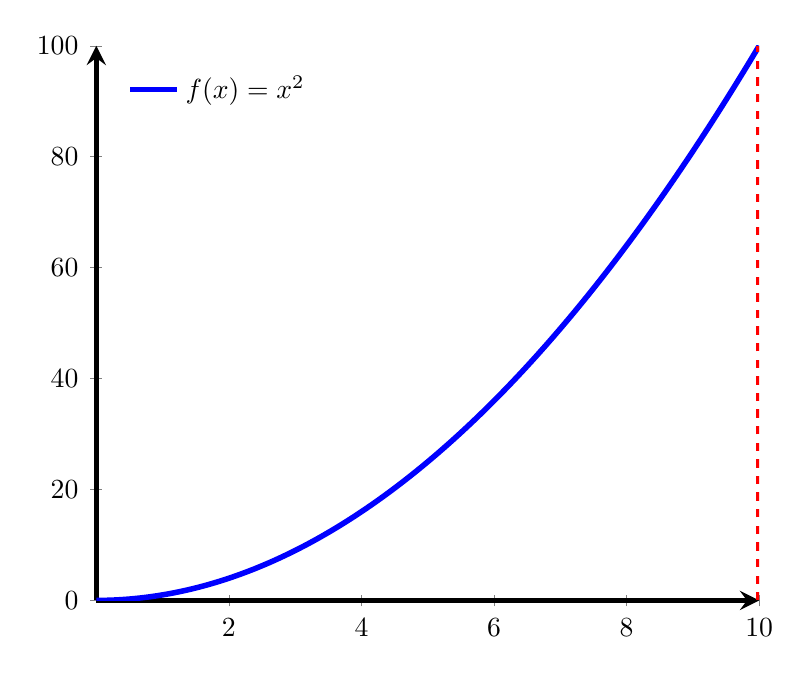
\begin{tikzpicture}
        \begin{axis}[axis lines=left, line width=2pt, xtick={2,4,6,8,10}, xticklabels={$2$,$4$,$6$,$8$,$10$}, legend entries= {$f(x)=x^2$},legend pos=north west,legend style={draw=none}]
            \addplot[samples=200, blue, domain=0:10]{x^2};
            \addplot[red, dashed] coordinates {(10,0) (10,100)};
        \end{axis}
    \end{tikzpicture}
    \\\\\colorbox{yellow}{Idea}: suddivido $[0,10]$ in tanti intervalli $[x_i,x_{i+1}]$ per $i=0,1,2,...,n-1$ quindi in $n$ intervalli
    con $x_0=0$ e $x_n=10$. Abbiamo quindi:\quad$0=x_0<x_1<x_2<\ ...\ <x_{n-1}<x_n=10$\\\\
    \begin{minipage}{0.5\textwidth}
    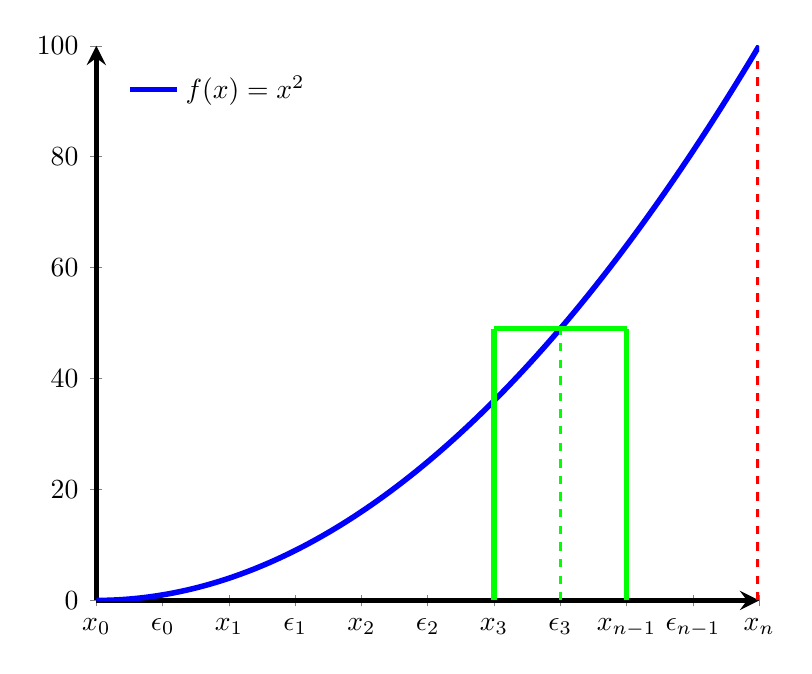
\begin{tikzpicture}
        \begin{axis}[axis lines=left, line width=2pt, xtick={0,1,2,3,4,5,6,7,8,9,10}, 
            xticklabels={$x_0$,$\epsilon_0$,$x_1$,$\epsilon_1$,$x_2$,$\epsilon_2$,$x_3$,$\epsilon_3$,$x_{n-1}$,$\epsilon_{n-1}$,$x_n$},
            legend entries= {,$f(x)=x^2$},legend pos=north west,legend style={draw=none}]
            \addplot[red, dashed] coordinates {(10,0) (10,100)};
            \addplot[samples=200, blue, domain=0:10]{x^2};
            \addplot[green, dashed, line width=1pt] coordinates {(7,0) (7,49)};
            \addplot[green] coordinates {(6,0) (6,49)};
            \addplot[green] coordinates {(8,0) (8,49)};
            \addplot[green] coordinates {(6,49) (8,49)};
        \end{axis}
    \end{tikzpicture}\end{minipage}\hfill
    \begin{minipage}{0.4\textwidth}
        \large Pe ogni $i=0,1,...,n-1$ prendo $\epsilon_i\in[x_i,x_{i+1}]$ e considero il rettangolo di base $[x_i,x_{i+1}]$ e altezza
        $f(\epsilon_i)=\epsilon_i^2$
    \end{minipage}\\\\
    Adesso generalizziamo questo ragionamento, unendo tutti i rettangoli, attraverso la sommatoria:
    \[\text{A}_{\text{tot}}=\sum_{i=0}^{n-1}(x_{i+1}-x_i)\cdot f(\epsilon_i)\]
    Per rappresentare questa sommatoria si usa \underline{l'integrale definito}:
    \[\text{A}_{\text{tot}}=\int_{0}^{10}f(x)\cdot dx=\int_{0}^{10}x^2\cdot dx\]\\
    \begin{defi}{Integrale di Cauchy-Riemann}{}
        Si dice partizione o suddivisione di $[a,b]$ un insieme finito di punti $\mathcal{P}=\{x_0,x_1,...,x_{n-1},x_n\}$ tale che
        \[a=x_0<x_1<\ ...\ <x_{n-1}<x_n=b\]
    \end{defi}
    \begin{defi}{Partizione Puntata}{}
        Si dice partizione puntata di $[a,b]$ una coppia $(\mathcal{P},\epsilon)$ dove $\mathcal{P}=\{x_0,x_1,...,x_{n-1},x_n\}$ è partizione
        di $[a,b]$ e $\epsilon=\{\epsilon_1,...,\epsilon_n\}$ con $\epsilon_k\in[x_{k-1},x_k]\quad\forall k=1,..,n$
    \end{defi}
    \colorbox{yellow}{Esempio}: $I=[0,1]\qquad\mathcal{P}_n=\{0,\frac1n,\frac2n,...,\frac{n-1}{n},1\}\qquad\mathcal{P} _4=\{0,\frac14,\frac12,\frac34,1\}$\\
    $\epsilon=\{\frac1{2n},\frac{1}{2n}+\frac{1}{n},...,\frac{1}{2n}+\frac{n-1}{n}\}\qquad$ Quindi $(\mathcal{P}_n,\epsilon)$ è una partizione puntata di $[0,1]$\\\\
    \begin{defi}{Integrale definito}{}
        Una funzione limitata $f:\ [a,b]\rightarrow\mathbb{R}$ si dice \underline{integrabile alla Cauchy-Riemann} in $[a,b]$
        se esiste $I\in\mathbb{R}$ tale che $\forall\epsilon>0\quad\exists\delta>0$ tale che $\forall(\mathcal{P}\epsilon)$ partizione puntata di 
        $[a,b]$ con $|\mathcal{P}|<\delta$ si ha\[|S(f,\mathcal{P},\epsilon)-I|<\delta\]
        Tale valore finito $I$ viene detto integrale definito di $f$ in $[a,b]$ e si indica:
        \[\int_{a}^{b}f(x)\cdot dx\]
    \end{defi}
    \colorbox{yellow}{Osservazione}: Per $S(f,\mathcal{P},\epsilon)$ si intende la somma puntata di $f$ rispetto alla partizione $(\mathcal{P},\epsilon)$ di $[a,b]$
    ossia: \[S(f,\mathcal{P},\epsilon)=\sum_{k=1}^{n}f(\epsilon_k)\cdot(x_k-x_{k-1})\]\\
    \colorbox{yellow}{Osservazione}: 
    \[\int_{a}^{a}f(x)\cdot dx=0\]
    \[\int_{a}^{b}f(x)\cdot dx= -\int_{b}^{a}f(x)\cdot dx\]\\
    \colorbox{yellow}{Osservazione}: Se $f$ è non negativa e integrabile, allora il suo integrale è l'area del sottografico
    definito da \[SG(f)=\{(x,y)\in\mathbb{R}^2:\quad0\le y\le f(x),\ x\in[a,b]\}\]\\
    \begin{theo}{}{}
        Sia $f:\ [a,b]\rightarrow\mathbb{R}$ monotona e limitata, allora $f$ è integrabile.\\
        Inotre $f$ è \underline{continua a tratti} se è continua tranne in un numero finito di punti, in cui ha
        limite destro e sinistro finiti, quindi discontinuità di prima specie.\\
        Le funzioni continue a tratti sono comunque integrabili, poichè basta sommare gli integrali nei vari tratti.
    \end{theo}
    \vspace{20pt}
    \begin{theo}{Proprietà dell'integrale}{}
        Sia $f,g;\ [a,b]\rightarrow\mathbb{R}$ integrabili. Allora:
        \begin{enumerate}
            \item Linearità dell'integrale: \[\int_{a}^{b}[\alpha f(x)+\beta g(x)]dx=\alpha\int_{a}^{b}f(x)\cdot dx+\beta\int_{a}^{b}g(x)\cdot dx\]
            \item Adattabilità rispetto all'insieme di integrazione: se $c\in[a,b]$
            \[\int_{a}^{b}f(x)\cdot dx=\int_{a}^{c}f(x)\cdot dx+\int_{c}^{b}f(x)\cdot dx\]
            \item Monotonia dell'integrale: se $f\le g$ in $[a,b]$
            \[\int_{a}^{b}f(x)\cdot dx\le\int_{a}^{b}f(x)\cdot dx\]
            \item Se $f$ è integrabile in $[a,b]$, allora anche $|f|$ lo è, e si ha:
            \[|\int_{a}^{b}f(x)\cdot dx|\le\int_{a}^{b}|f(x)|\cdot dx\]
        \end{enumerate}
    \end{theo}
    \vspace{20pt}
    \begin{theo}{Media integrale}{}
        Sia $f:\ [a,b]\rightarrow\mathbb{R}$ integrabile e continua per Weistrass esiste $m=\text{inf }f,\quad M=\text{supp }f$ allora:
        \[m\le\frac{1}{b-a}\int_{a}^{b}f(x)\cdot dx\le M\]
        Se $f$ è continua in $[a,b]$ allora esiste $c\in[a,b]$ tale che
        \[\frac{1}{b-a}\int_{a}^{b}f(x)dx=f(c)\]
    \end{theo}
    \colorbox{yellow}{Dim}: sapendo che $m\le f(x)\le M\qquad\forall x\in[a,b]$
    \begin{align*}
        &\Rightarrow\qquad\int_{a}^{b}m\cdot dx\le\int_{a}^{b}f(x)\cdot dx\le\int_{a}^{b}M\cdot dx&&&&&\\
        &\Rightarrow\qquad\int_{a}^{b}m\cdot dx=m\cdot\int_{a}^{b}1\cdot dx=m\cdot(b-a)\\
        &\Rightarrow\qquad m\cdot(b-a)\le\int_{a}^{b}f(x)\cdot dx\le M\cdot(b-a)\\
        &\Rightarrow\qquad m\le\frac{1}{b-a}\cdot\int_{a}^{b}f(x)\cdot dx\le M
    \end{align*}
    Se $f$ è continua $f([a,b])=[m,M]$\quad ed esiste $c\in[a,b]$ tale che \[f(c)=\frac{1}{b-a}\int_{a}^{b}f(x)\ dx\]\\
    \colorbox{yellow}{Osservazione}: se $f$ non è continua, potrebbe non esistere $c\in[a,b]$ poichè il teorema di Weistrass
    non assicura massimo e minimo per funzioni non continue.\\\\
    \begin{defi}{Primitiva e famiglia di primitive}{}
        Sia $A\subseteq\mathbb{R},\ f:\ A\rightarrow\mathbb{R}$ una funzione $F:\ A\rightarrow\mathbb{R}$ si dice
        \underline{primitiva di $f$} o funzione primitiva di $f$ in $A$ se $F$ è derivabile in $A$ e si ha
        \[F'(x)=f(x)\qquad\forall x\in A\]
        La \underline{famiglia di primitive} è invece l'unione di tutte le $F(x)$ la cui derivata prima è uguale $f(x)$
        con l'aggiunta di una costante $c$
    \end{defi}
    \colorbox{yellow}{Esempio}: se $f$ è derivabile, allora $f$ è una primitiva di $f'$\\
    $\int f(x)\cdot dx=F(x)+c$ quindi $F(x)+c$ è la famiglia di primitive di $f(x)$\\\\
    \begin{theo}{}{}
        Siano $F,G$ due primitive di $f$ sia $A=I$ intervallo. Allora esiste $c\in\mathbb{R}$ tale che\[F(x)=G(x)+c\qquad\forall x\in I\]
    \end{theo}
    \colorbox{yellow}{Dim}: so che $G'(x)=f(x)=F'(x)\quad\forall x\in I$
    \begin{align*}
        &\Rightarrow\quad\left(F(x)-G(x)\right)'=F'(x)-G'(x)=f(x)-f(x)=0&&&&&&\\
        &\Rightarrow\quad F-G\quad\text{ è costante in }I\\
        &\Rightarrow\quad\exists\ c\in\mathbb{R}\quad\text{tale che}\quad F(x)-G(x)=c\quad\forall x\in I\\
        &\Rightarrow\quad\exists\ c\in\mathbb{R}\quad\text{tale che}\quad F(x)=G(x)-c\quad\forall x\in I\quad\checkmark\\
    \end{align*}
    \begin{theo}{Teorema fondamentale del calcolo 1° parte}{}
        Se $f\in C°[a,b]$ e definisco \[F(x)=\int_{a}^{x}f(t)\ dt\qquad\forall x\in[a,b]\]
        allora $F$ è derivabile (e continua) in $[a,b]$ e si ha $F'(x)=f(x)$ quindi $F$ è primitiva di $f$
    \end{theo}\vspace{20pt}
    \begin{theo}{2° parte calcolo fondamentale}{}
        Sia $f(x)$ continua in $[a,b]$ e sia $F(x)$ una sua qualsiasi primitiva in $[a,b]$. Allora:
        \[F(b)-F(a)=\int_{a}^{b}f(x)\ dx\]
    \end{theo}
    \colorbox{yellow}{Dim}: Dalla prima parte del teorema sappiamo che la funzione integrale nel punto $a$ è una primitiva
    della funzione stessa e quindi qualsiasi altra primitiva nell'intervallo $[a,b]$ è diversa dalle altre per un valore finito
    $c\in\mathbb{R}$. Quindi:\[F(x)=\int_{a}^{x}f(t)\ dt+c\]
    Otteniamo quindi che: \[F(b)-F(a)=(\int_{a}^{b}f(t)\ dt+c)-(\int_{a}^{a}f(t)\ dt+c)=\int_{a}^{b}f(t)\ dt\]
    La variabile di integrazione è indifferente quindi possiamo sostituire $t$ con $x$ ed abbiamo verificato la nostra tesi.\\\\
    \begin{defi}{Integrale indefinito}{}
        Data una funzione $f:\ A\rightarrow\mathbb{R}$ l'integrale indefinito di $f$ in $A$ è l'insieme di tutte le sue
        primitive in $A$ e si denota\[\int f(x)\ dx=\{F:\ F\text{ è primitiva di $f$ in $A$}\}\]
        Se $A$ è un intervallo, allora\[\int f(x)\ dx=\{F+c:\ c\in\mathbb{R}\}\]
    \end{defi}
    \colorbox{yellow}{Osservazione}: l'integrale indefinito è lineare, ossia:\[\int f(x)+g(x)\ dx=\int f(x)\ dx+\int g(x)\ dx\]\\
    \subsection{Metodi di integrazione}
    \begin{defi}{Integrazione per parti}{}
        Siano $f,g$ funzioni derivabili in $I=[a,b]$, allora:
        \[(f(x)\cdot g(x))'=f'(x)\cdot g(x)+f(x)\cdot g'(x)\qquad\forall x\in[a,b]\]
        Quindi, integrando:\[\int_{a}^{b}f'(x)\cdot g(x)\ dx= [f(x)\cdot g(x)]^b_a-\int_{a}^{b}f(x)\cdot g'(x)\ dx\]
    \end{defi}\vspace{20pt}
    \begin{defi}{Integrazione per sostituzione}{}
        $f:\ [a,b]\rightarrow\mathbb{R}$ continua, $\varphi:\ [c,d]\rightarrow[a,b]$ di classe $C^1$ e tale che $\varphi(c)=a$,
        $\varphi(d)=b$, $F$ primitiva di $f$ in $[a,b]$. Allora:
        \[\int_{c}^{d}f(\varphi(t))\cdot\varphi'(t)\ dt=\int_{a}^{b}f(x)\ dx\]
    \end{defi}\vspace{20pt}
    \begin{ex}{}{}
        \[\int (e^{3x}-\frac{1}{x^3}+\frac{1}{x\cdot(1+\ln^2x)})\ dx\]
    \end{ex}
    \colorbox{yellow}{Svolgimento}:
    \begin{align*}
        &\Rightarrow\qquad\int e^{3x}-\int\frac{1}{x^3}+\int\frac{1}{x\cdot(1+\ln^2x)} &&&&&&&&\\
        &\Rightarrow\qquad\frac{1}{3}\int\underbrace{3}_{f'(x)}\cdot e^{3x}\ dx\quad+\frac{1}{2x^2}\quad+\int\frac{1}{x\cdot(1+\ln^2x)}\\
        &\Rightarrow\qquad\frac{e^{3x}}{3}+\frac{1}{2x^2}+\quad\int\frac{1}{x}\cdot\frac{1}{1+(\ln x)^2}\\
        &\text{Quindi: }\quad\int f'(x)\cdot f(x)\\
        &\Rightarrow\qquad\frac{e^{3x}}{3}+\frac{1}{2x^2}+\arctan(\ln x)+c
    \end{align*}
    \begin{defi}{Integrale di funzione razionale}{}
        Consideriamo l'integrale:\[\int \frac{\mathcal{P}(x)}{\mathcal{Q}(x)}\ dx\qquad\text{ con }\mathcal{P}\text{ e }\mathcal{Q}\text{ polinomi}\]
        L'idea è riscrivere l'integrale come la somma di due integrali di cui riusciamo a calcolare la primitiva e abbiamo tre casi:
        \begin{enumerate}
            \item $\Delta>0$ e $(x-x_1)\cdot(x-x_2)=x^2+cx+d$\[\int\frac{ax+b}{x^2+cx+d}=\int\frac{A}{x-x_1}+\int\frac{B}{x-x_2}\]
            \item $\Delta=0$ e $(x-x_1)^2=x^2+cx+d$\[\int\frac{ax+b}{x^2+cx+d}=\int\frac{A}{x-x_1}+\int\frac{B}{(x-x_1)^2}\]
            \item $\Delta<0$ \[\int\frac{ax+b}{x^2+cx+d}=\frac a2\int\frac{\overbrace{2x+c}^{f'(x)}}{\underbrace{x^2+cx+d}_{f(x)}}+b\int\frac{1}{x^2+cx+d}\]
        \end{enumerate}
    \end{defi}
    \vspace{10pt}\begin{ex}{Caso 1}{}
        \[\int\frac{3x+2}{x^2-5x+6}\]
    \end{ex}
    \colorbox{yellow}{Svolgimento}: visto che $\Delta>0$ allora posso applicare il primo caso:
    \begin{align*}
        &x_1=3\quad x_2=2\qquad\Rightarrow\qquad x^2-5x+6=(x-2)\cdot(x-3)&&&&&&&&\\
        &\Rightarrow\qquad\frac{A}{x-2}+\frac{B}{x-3}\\
        &\ Ax+Bx=3x\brace -3A-2B=2\ \\
        &\text{Risolvendo il sistema otteniamo che: }\quad A=-8\quad B=11\\
        &\int\frac{3x+2}{x^2-5x+6}\quad\Rightarrow\quad\int\frac{-8}{x-2}dx+\int\frac{11}{x-3}dx\\
        &\Rightarrow\qquad-8\ln|x-2|+11\ln|x-3|+c\\\\
    \end{align*}
    \begin{ex}{Caso 2}{}
        \[\int\frac{x+2}{(x-2)^2}\]
    \end{ex}
    \colorbox{yellow}{Svolgimento}: visto che $\Delta=0$ applichiamo il secondo caso:
    \begin{align*}
        &\Rightarrow\qquad\frac{A}{x-2}+\frac{B}{(x-2)^2}&&&&&&&&&\\
        &Ax=x\brace-2A+B=2\\
        &\text{Risolvendo il sistema otteniamo che: }\quad A=1\quad B=4\\
        &\int\frac{x+2}{(x-2)^2}\quad\Rightarrow\quad\int\frac{1}{x-2}dx+\int\frac{4}{(x-2)^2}dx\\
        &\Rightarrow\quad\ln|x-2|-\frac{4}{x-2}+c\\\\
    \end{align*}
    \begin{ex}{Caso 3}{}
        \[\int\frac{3x+2}{x^2+4x+5}\]
    \end{ex}
    \colorbox{yellow}{Svolgimento}: visto che $\Delta<0$ applichiamo il terzo caso:
    \begin{align*}
        &\Rightarrow\quad3\int\frac{x}{x^2+4x+5}dx+2\int\frac{1}{x^2+4x+5}dx&&&&&&&&\\
        &\Rightarrow\quad\frac{3}{2}\int\frac{\overbrace{2x+4}^{f'(x)}-4}{\underbrace{x^2+4x+5}_{f(x)}}dx+2\int\frac{1}{1+(x+2)^2}dx\\
        &\Rightarrow\quad\frac{3}{2}\ln|x^2+4x+5|\qquad-4\cdot\frac{3}{2}\int\frac{1}{1+(x+2)^2}dx+2\int\frac{1}{1+(x+2)^2}dx\\
        &\Rightarrow\quad\frac{3}{2}\ln(x^2+4x+5)-4\arctan(x+2)+c\\\\
    \end{align*}
    \subsection{Integrale improprio}
    \begin{defi}{Integrale generalizzato o improprio}{}
        Può capitare di avere $f:\ I\rightarrow\mathbb{R}$ con $f$ o $I$ o entrambi illimitati, ma vogliamo calcolare comunque un'area (o integrale).\\
        Sia $f:\ (a,b]\rightarrow\mathbb{R}$ integrabile in $[c,d]\quad\forall c\in\ (a,b]$. Se esiste:
        \[\lim_{c\rightarrow a^+}\int_{c}^{b}f(x)\cdot dx\]
        Tale limite si chiama \underline{integrale improprio o generalizzato} di $f$ in $[a,b]$.\\\\
        Se il limite esiste finito, si dice che $f$ è integrabile in \underline{senso generalizzato} e l'integrale si dice convergente,
        altrimenti si dice che l'integrale è divergente.
    \end{defi}
    \colorbox{yellow}{Osservazione}: se $|f|$ è integrabile in senso improprio si dice che $f$ è 
    \underline{assolutamente integrabile in senso} \underline{improprio} e:\[|\int_a^bf(x)\ dx|\le\int_{a}^{b}f(x)\ dx\]\\
    \begin{ex}{}{}
        \[\int_{0}^{1}\frac{1}{\sqrt{x}}\ dx\]
    \end{ex}
    \colorbox{yellow}{Svolgimento}: ci accorgiamo che $0$ non fa parte del dominio di $f$ quindi dobbiamo fare:
    \[\lim_{c\rightarrow0^+}\int_{c}^{1}\frac{1}{\sqrt{x}}dx=\lim_{c\rightarrow0^+}2-\frac{\sqrt{x}}{2}=2\]\\
    \begin{theo}{Teorema del Confronto}{}
        Siano $f,g:\ (a,b]\rightarrow\mathbb{R}\quad a\in\mathbb{\bar R}$ con $f,g$ integrabili in $[c,b]\quad\forall c\in]a,b[$ tale che:
        \[0\le f(x)\le g(x)\qquad\forall x\in(a,b]\]
        Allora:
        \begin{itemize}
            \item $\int g(x)\ dx<+\infty\quad\Rightarrow\quad\int f(x)\ dx<+\infty$
            \item $\int f(x)\ dx=+\infty\quad\Rightarrow\quad\int g(x)\ dx=+\infty$
        \end{itemize}
    \end{theo}
    \vspace{20pt}\begin{theo}{Criterio asintotico del Confronto}{}
        $f,g:\ (a,b]\rightarrow\mathbb{R}$ integrabili in $[c,b]\quad\forall c\in]a,b[$ tale che:
        \[\lim_{x\rightarrow a^+}|\frac{f(x)}{g(x)}|=l\]\\
        \begin{enumerate}
            \item se $l\in\mathbb{R}\smallsetminus\{0\}$ allora $f$ è ass. integrabile in $(a,b]$ se e solo se lo è anche $g$ nello stesso intervallo
            \item se $l=0$ allora se $g$ è ass. integrabile in $(a,b]$, allora lo è anche $f$
            \item se $l=+\infty$ allora se l'integrale da $a$ a $b$ di $|g(x)|=+\infty$ allora anche lo stesso integrale per $|f(X)|=+\infty$ 
        \end{enumerate}
    \end{theo}
    \colorbox{yellow}{Osservazione}: è importante avere funzioni di cui conosciamo l'integrabilità.\\\\
    \begin{theo}{Criterio integrale per le serie}{}
        $f:\ [k_0,+\infty[\ \rightarrow[0,+\infty[,$ decrescente$,\ k_0\in\mathbb{N}$. Allora:
        \[\sum_{k=k_0}^{+\infty}f(x)<+\infty\quad\Leftrightarrow\quad\int_{k_0}^{+\infty}f(x)\ dx<+\infty\]
    \end{theo}
    \colorbox{yellow}{Esempio casi importanti}:
    \[\int_{0}^{1}\frac{1}{x^\alpha}<+\infty\quad\Leftrightarrow\quad\alpha<1\]Se $\alpha\ge1$ allora $\Rightarrow+\infty$
    \[\int_{1}^{+\infty}\frac{1}{x^\alpha}<+\infty\quad\Leftrightarrow\quad\alpha>1\]Se $\alpha\le1$ allora $\Rightarrow+\infty$\\\\
    \colorbox{yellow}{Osservazione}:\[\int_{0}^{+\infty}\frac{1}{x^\alpha}=\int_{0}^{1}\frac{1}{x^\alpha}+\int_{1}^{+\infty}\frac{1}{x^\alpha}=+\infty\qquad\forall\alpha\in\mathbb{R}\]
    \newpage\section{Equazioni Differenziali}
    \vspace{10pt}
    \begin{defi}{Equazione differenziale}{}
        Un'equazione differenziale è un'equazione che esprime una relazione tra due funzioni e le sue derivate fino ad un certo ordine.
        \[F\left(t,y(t), y'(t),\dots,y^{(n)}(t)\right)=0\qquad\circledast\]
        Cerco una $f.\ y(t)$ derivabile $n$ volte che soddisfi l'equazione $\circledast$
    \end{defi}
    Considero il Problema di Cauchy:\\
    \begin{minipage}{0.4\textwidth}
        \begin{center}
            (PC)
        \end{center}
    \end{minipage}\hfill
    \begin{minipage}{0.05\textwidth}
        \Huge$\left\{\right.$
    \end{minipage}
    \begin{minipage}{0.2\textwidth}
        $y'=f(t,y)$\\\\
        $y(t_0)=y_0$
    \end{minipage}
    \begin{minipage}{0.2\textwidth}
        equazione differenziale del primo ordine in forma normale (ED)\\\\
        dato o condizione iniziale (C.I.)
    \end{minipage}\\\\
    \begin{theo}{Teorema di Cauchy Lipschitz}{}
        Considero il (PC). Suppongo che esistano due intervalli aperti $I,J$ con $A\in I$ e $y_0\in J$ tale che
        \[f_\shortmid\frac{a\ f}{a\ y}\qquad\text{siano continue}\]
        Allora esiste $\tilde{I}$ intorno di $t_0$ tale che (PC) ammette un'unica soluzione $y:\ \tilde{I}\rightarrow\mathbb{R}$.
    \end{theo}
    \colorbox{yellow}{Osservazione}: dire che esiste una soluzione $\ne$ da dire che è determinata.\\
    In generale (PC) e (ED) non si risolvono esplicitamente. Noi vediamo i casi in cui si possono risolvere.\\\\
    \begin{defi}{Equazione differenziale di 1° ordine}{}
        Un'equazione differenziale del 1° ordine in forma normale è un'equazione del tipo:
        \[y'=a(t)\ y+b(t)\]
        Dove $a(t)$ e $b(t)$ sono due funzioni $a,b:\ I\rightarrow\mathbb{R}$. Una soluzione è
        \[y'(t)=a(t)\ y(t)+b(t)\qquad\forall t\in I\]
        L'insieme di tutte le soluzioni si chiama \underline{integrale generale}.
    \end{defi}
    \vspace{20pt}
    \begin{ex}{}{}
        \[y'=3y\]
    \end{ex}
    \colorbox{yellow}{Svolgimento}: La funzione $y(t)=e^{3t}$ è una soluzione. Infatti $y'(t)=3e^{3t}=3y(t)$\\
    $\Rightarrow\qquad y(t)=e^{3t}$ soddisfa l'equazione.\\
    Se prendo $y(t)=K\cdot e^{3t}$ ho l'integrale generale di $y'(t)=3y$\\\\
    \begin{ex}{Lineari}{}
        \[y'=3y+t\]
    \end{ex}
    \colorbox{yellow}{Svolgimento}: $y'=a(t)\cdot y+b(t)$
    \begin{align*}
        &a(t)=3\qquad b(t)=t\qquad a,b:\ \mathbb{R}\rightarrow\mathbb{R} &&&&&\\
        &A(t) = 3t\\
        &\Rightarrow\quad y(t)=e^{3t}\cdot\left(\int t\cdot e^{-3t}\ dt\right)\qquad\text{ utilizzato la formula di risoluzione delle ED lineari}\\
        &\Rightarrow\quad y(t)=e^{3t}\cdot\left(-\frac13e^{-3t}\cdot t-\frac19e^{-3t}+c\right)\\
        &\Rightarrow\quad y(t)=-\frac t3-\frac19+c\ e^{3t}\qquad c\in\mathbb{R}
    \end{align*}
    Posso verificare che sia la soluzione derivando $y(t)$\\\\
    \begin{ex}{A variabili separabili}{}
        \[y'=t\cdot y^2\]
    \end{ex}
    \colorbox{yellow}{Svolgimento}: $a(t)=t\quad b(y)=y^2$\\\\
    Cerco le soluzioni costanti, quindi con $b(\bar{y})=0$ ossia $\bar{y}^2=0\quad\Rightarrow\quad\bar{y}=0$\\
    L'unica soluzione costante è quindi $y(t)=0$.\\\\
    Adesso cerco le soluzioni non costanti:$\qquad$ Se $y(t)\ne0$ posso dividere per $\left(y(t)\right)^2$
    \[\frac{y'(t)}{\left(y(t)\right)^2}=t\]
    Da cui:
    \begin{align*}
        &\Rightarrow\quad\int\frac{y'(t)}{(y(t))^2}\ dt=\int t\ dt&&\\
        &\Rightarrow\quad\int\frac{1}{s^2}\ ds=\frac{t^2}{2}+c\qquad s=y(t)\\
        &\Rightarrow\quad-\frac{1}{s}=\frac{t^2}2+c\qquad s=y(t)\\
        &\Rightarrow\quad y(t)=-\frac{1}{\frac{1}{2}t^2+c}
    \end{align*}
    \newpage\section{Tabelle Utili}
    \vspace{10pt}
    \subsection{Proprietà potenze e logaritmi}\vspace{5pt}\large
    \begin{center}
        \rowcolors{1}{gray!8}{white!100}
        \begin{tabular}{| c | c |}
            \hline
            $a^m\cdot a^n=a^{m+n}$ & $a^m\cdot b^m=(a\cdot b)^m$\\\hline
            $\frac{a^m}{a^n}=a^{m-n}$ & $\frac{a^m}{b^m}=\left(\frac ab\right)^m$\\\hline
            $\left(a^m\right)^n=a^{m\cdot n}$ & /\\\hline
            $a^{\log_a(b)}=b$ & $\log_a(b\cdot c)=\log_a(b)+\log_a(c)$\\\hline
            $\log_a(b^c)=c\cdot\log_a(b)$ & $\log_a\left(\frac bc\right)=\log_a(b)-\log_a(c)$\\\hline
            $\log_a(b)=\frac{\log_c(b)}{\log_c(a)}$ & $\log_a(b)=\frac{1}{\log_b(a)}$\\\hline
        \end{tabular}
    \end{center}
    \vspace{10pt}
    \subsection{Limiti notevoli}\vspace{5pt}\large
    \begin{center}
        \rowcolors{1}{gray!8}{white!100}
        \begin{tabular}{| c | c |}
            \hline
            $\lim_{x\rightarrow0}\frac{\sin x}x=1$ & $\lim_{x\rightarrow0}\frac{\tan x}{x}=1$\\\hline
            $\lim_{x\rightarrow0}\frac{1-\cos x}x=0$ & $\lim_{x\rightarrow0}\frac{\arcsin x}{x}=1$\\\hline
            $\lim_{x\rightarrow0}\frac{1-\cos x}{x^2}=\frac12$ & $\lim_{x\rightarrow0}\frac{\arctan x}{x}=1$\\\hline
            $\lim_{x\rightarrow+\infty}\left(1+\frac1x\right)^x=e  $ & $\lim_{x\rightarrow0}\left(1+x\right)^{\frac1x}=e$\\\hline
            $\lim_{x\rightarrow0}\frac{\log_a(1+x)}x=\log_ae$ & $\lim_{x\rightarrow0}\frac{\ln(1+x)}{x}=1$\\\hline
            $\lim_{x\rightarrow0}\frac{a^x-1}x=\ln a$ & $\lim_{x\rightarrow0}\frac{e^x-1}{x}=1$\\\hline
            $\lim_{x\rightarrow0}\frac{(1+x)^k-1}x=k$ & $\lim_{x\rightarrow+\infty}\frac{x^n}{a^x}=0\quad a>0$\\\hline
            $\lim_{x\rightarrow0^+}x^a\cdot\log_ax=0\quad a>0,a>1$ & / \\\hline
        \end{tabular}
    \end{center}
    \vspace{10pt}
    \subsection{Sviluppi asintotici di alcune funzioni}\vspace{5pt}\large
    \begin{center}
        \rowcolors{1}{gray!8}{white!100}
        \begin{tabular}{| c | c |}
            \hline
            $\sin x$ & $x-\frac{x^3}{3!}+\frac{x^5}{5!}+o(x^5)$ per $x\rightarrow0$\\\hline
            $\cos x$ & $1-\frac{x^2}{2!}+\frac{x^4}{4!}+o(x^4)$ per $x\rightarrow0$\\\hline
            $\ln(1+x)$ & $x-\frac{x^2}{2}+\frac{x^3}{3}+o(x^3)$ per $x\rightarrow0$\\\hline
            $\cosh x$ & $1-\frac{x^2}{2!}+\frac{x^4}{4!}+o(x^4)$ per $x\rightarrow0$\\\hline
            $\sinh x$ & $x-\frac{x^3}{3!}+\frac{x^5}{5!}+o(x^5)$ per $x\rightarrow0$\\\hline
            $\tan x$ & $x+\frac{x^3}{3}+o(x^3)$ per $x\rightarrow0$\\\hline
            $\arctan x$ & $x-\frac{x^3}{3}+o(x^3)$ per $x\rightarrow0$\\\hline
            $e^x$ & $1+x+\frac{x^2}{2!}+\frac{x^3}{3!}+o(x^3)$\\\hline
        \end{tabular}
    \end{center}
    \subsection{Tabella Derivate Semplici}\vspace{5pt}\begin{center}\large
        {\rowcolors{1}{gray!8}{white!100}
        \begin{tabular}{| c | c |}
            \hline
            \LARGE f(x) &\LARGE f$^\text{1}$(x)\\\hline
            $k$ & $0$\\\hline
            $x^n$ & $n\cdot x^{n-1}$\\\hline
            $\ln |x|$ & $\frac{1}{x}$\\\hline
            $\log_a |x|$ & $(\log_ae)\cdot\frac{1}{x}$\\\hline
            $e^x$ & $e^x$\\\hline
            $a^x$ & $(\ln a)\cdot a^x$\\\hline
            $\sin x$ & $\cos x$\\\hline
            $\cos x$ & $-\sin x$\\\hline
            $\tan x$ & $\frac{1}{\cos^2x}=1+\tan^2x$\\\hline
            $\cot x$ & $-\frac{1}{\sin^2x}=-1-\cot^2x$\\\hline
            $\arcsin x$ & $\frac{1}{\sqrt{1-x^2}}$\\\hline
            $\arccos x$ & $-\frac{1}{\sqrt{1-x^"}}$\\\hline
            $\arctan x$ & $\frac{1}{1+x^2}$\\\hline
        \end{tabular}}
    \end{center}
       \subsection{Sviluppi di McLaurin}\vspace{5pt}\large\begin{center}
        {\rowcolors{1}{gray!8}{white!100}
        \begin{tabular}{| c | c | c |}
            \hline
            \LARGE f(x) &\LARGE P$^n_0(x)$&\LARGE $\sum_{k=0}^{n\rightarrow+\infty}$\\\hline
            $e^x$ per $x\rightarrow 0$ &$1+x+\frac{x^2}{2!}+\frac{x^3}{3!}+\dots$& $\sum\frac{x^k}{k!}+o(x^k)$\\\hline
            $\log(1+x)$ per $x\rightarrow 0$ &$x+-\frac{x^2}{2}+\frac{x^3}{3}+\frac{x^3}{3!}+\dots$& $\sum(-1)^{k+1}\frac{x^k}{k}+o(x^k)$\\\hline
            $(1+x)^\alpha$ per $x\rightarrow 0$ &$1+\alpha x+\frac{\alpha(\alpha-1)x^2}{2}+\dots$& $\sum\binom{\alpha}{k}x^k+o(x^k)$\\\hline
            $\cos x$ per $x\rightarrow 0$ &$1-\frac{x^2}{2!}+\frac{x^4}{4!}-\dots$& $\sum(-1)^{k}\frac{x^{2k}}{(2k)!}+o(x^{2k})$\\\hline
            $\cosh x$ per $x\rightarrow 0$ &$1+\frac{x^2}{2!}+\frac{x^4}{4!}+\dots$& \\\hline
            $\sin x$ per $x\rightarrow 0$ &$x-\frac{x^3}{3!}+\frac{x^5}{5!}-\dots$& $\sum(-1)^{k}\frac{x^{2k+1}}{(2k+1)!}+o(x^{2k+1})$\\\hline
            $\sinh x$ per $x\rightarrow 0$ &$x+\frac{x^3}{3!}+\frac{x^5}{5!}+\dots$& \\\hline
            $\arctan x$ per $x\rightarrow 0$ &$x-\frac{x^3}{3}+\frac{x^5}{5}-\dots$& $\sum(-1)^{k}\frac{x^{2k+1}}{2k+1}+o(x^{2k+1})$\\\hline
            $\tan x$ per $x\rightarrow 0$ &$x+\frac{x^3}{3}+\frac{2x^5}{15}+\dots$& \\\hline
        \end{tabular}}
    \end{center}
            \subsection{Integrali indefiniti noti}\vspace{5pt}\large\begin{center}
        {\rowcolors{1}{gray!8}{white!100}
        \begin{tabular}{| c | c |}
            \hline
            \LARGE$\int f(x)$ & \LARGE$F(x)$\\\hline
            $\int e^x\ dx$ & $e^x+c$\\\hline
            $\int x^\alpha\ dx$ & $\frac{1}{\alpha+1}\cdot x^{\alpha+1}+c$\\\hline
            $\int \frac{1}{x}\ dx$ & $\ln|x|+c$\\\hline
            $\int \alpha^x\ dx$ & $\frac{1}{\ln\alpha}\cdot\alpha^x+c$\\\hline
            $\int \sin x\ dx$ & $-\cos x+c$\\\hline
            $\int \cos x\ dx$ & $\sin x+c$\\\hline
            $\int \frac{1}{\cos^2x}\ dx$ & $\tan x+c$\\\hline
            $\int \frac{1}{1+x^2}\ dx$ & $\arctan x+c$\\\hline
            $\int \frac{1}{\sin^2x}\ dx$ & $-\cot x+c$\\\hline
            $\int \frac{1}{\sqrt{1-x^2}}\ dx$ & $\arcsin x+c$\\\hline
        \end{tabular}}
    \end{center}
                \subsection{Come risolvere le Equazioni Differenziali}\vspace{5pt}\large\begin{center}
        {\rowcolors{1}{gray!8}{white!100}
        \begin{tabular}{| c | c |}
            \hline
            \LARGE ED & \LARGE $y'=a(t)\cdot y+b(t)$\\\hline
            $y'=b(t)\qquad a(t)=0$ & $\int b(t)=B(t)+c$\\\hline
            $y'(t)=a(t)\cdot b(y(t))$ & $\int\frac{y'(t)}{b(y(t))}\ dt=\int a(t)\ dt$\\\hline
            $y'=a(t)\cdot y+b(t)$ & $y=e^{A(t)}\cdot\int e^{-A(t)}\cdot b(t)\ dt\qquad A(t)=\int a(t)\ dt$\\\hline
        \end{tabular}}
    \end{center}
\end{document}
